\documentclass[12pt,a4paper,oneside]{report}

% =========================================================
% SYSTEM PACKAGES & CONFIGURATIONS
% =========================================================
\usepackage[left=1.5in, right=1.0in, top=1.0in, bottom=1.0in]{geometry}
\usepackage{mathptmx} % Times New Roman Font Emulation
\usepackage{setspace}
\usepackage{amsmath,amssymb,amsfonts}
\usepackage{graphicx}
\usepackage{booktabs}
\usepackage{multirow}
\usepackage{caption}
\usepackage{subcaption}
\usepackage{url}
\usepackage{tikz}
\usepackage{titlesec}
\usepackage{indentfirst}
\usepackage{float}
\usepackage{xcolor}

\usetikzlibrary{shapes.geometric, arrows.meta, positioning, calc}

% Enforce Paragraph Spacing Rules (6pt Before & 6pt After)
\setlength{\parskip}{6pt}
\setlength{\parindent}{0.5in}
\setstretch{1.5} % 1.5 Line Spacing for General Text
\emergencystretch=1em % Automatically resolves overfull \hbox margin warnings

% =========================================================
% TYPOGRAPHY & HIERARCHY MATRICES (INSTITUTIONAL SPECS)
% =========================================================
\titleformat{\chapter}[display]
  {\normalfont\fontsize{15}{15}\bfseries\centering}{\MakeUppercase{\chaptertitlename\ \thechapter}}{10pt}{}
\titlespacing*{\chapter}{0pt}{20pt}{20pt}

\titleformat{\section}
  {\normalfont\fontsize{12}{12}\bfseries}{\thesection}{1em}{\MakeUppercase}
\titlespacing*{\section}{0pt}{12pt}{6pt}

\titleformat{\subsection}
  {\normalfont\fontsize{12}{12}\bfseries}{\thesubsection}{1em}{}
\titlespacing*{\subsection}{0pt}{12pt}{6pt}

% Caption Customization
\captionsetup[table]{labelfont=normalfont, textfont=normalfont, labelsep=space, justification=centering, singlelinecheck=false, position=top}
\captionsetup[figure]{labelfont=normalfont, textfont=normalfont, labelsep=period, justification=centering, position=bottom}

\begin{document}

% =========================================================
% PRELIMINARY PAGES (ROMAN NUMERAL NUMBERING)
% =========================================================
\pagenumbering{roman}

% Exact Palette Calibration based on the user's screenshots
\definecolor{scetblue}{RGB}{28, 54, 115}   % Dark Royal/Navy Blue for Institutional Headers
\definecolor{scetred}{RGB}{255, 0, 0}      % Pure Primary Red for Degree/University Details
\definecolor{scetgreen}{RGB}{0, 153, 76}   % Forest Green for Submission Phrases
\definecolor{scetorange}{RGB}{230, 100, 0} % Golden/Orange for Candidate Details
\definecolor{scetpurple}{RGB}{120, 30, 120} % Purple for External Examiner
\definecolor{textblue}{RGB}{0, 102, 204}   % Bright Blue for Project Title in Certificate
\definecolor{textred}{RGB}{220, 30, 30}    % Red for Certificate Text
\definecolor{textgreen}{RGB}{0, 153, 76}   % Green for Student Name/Roll Number in Certificate
\definecolor{scetbrown}{RGB}{139, 69, 19}  % Saddle Brown for Signature Headers

% ---------------------------------------------------------
% 1. COVER PAGE (STRICT 1-PAGE PERFECTLY BALANCED LAYOUT)
% ---------------------------------------------------------
\begin{titlepage}
\newgeometry{left=1.5in, right=1.0in, top=0.8in, bottom=0.8in}
\setlength{\parskip}{4pt}
\begin{center}
    \vspace*{0.15in}
    \setstretch{1.1}
    
    % MAIN TITLE (All Caps, Black, Prominent font size)
    {\fontsize{18}{22}\bfseries\selectfont\color{black} BEYOND THE PRIVACY-UTILITY TRADE-OFF: A SPATIOTEMPORAL-CONSTRAINT AND SECURE INTELLIGENT CAMPUS MONITORING SYSTEM\par}
    
    \vspace{0.2in}
    % REPORT LEVEL (ALL CAPS - Red)
    {\fontsize{12}{14}\bfseries\selectfont\color{scetred} A PROJECT REPORT\par}
    \vspace{0.02in}
    {\fontsize{10}{12}\itshape\selectfont\color{scetgreen} Submitted in partial fulfillment of the requirements to\par}
    
    \vspace{0.05in}
    % UNIVERSITY SPECIFICATION (ALL CAPS - Red)
    {\fontsize{13}{15}\bfseries\selectfont\color{scetred} JAWAHARLAL NEHRU TECHNOLOGICAL UNIVERSITY KAKINADA\par}
    \vspace{0.02in}
    {\fontsize{10}{12}\itshape\selectfont\color{scetgreen} For the award of the degree of\par}
    
    \vspace{0.05in}
    % ACADEMIC DEGREE BLOCK (ALL CAPS - Red)
    {\fontsize{14}{16}\bfseries\selectfont\color{scetred} MASTER OF TECHNOLOGY\par}
    \vspace{0.02in}
    {\fontsize{10}{12}\itshape\bfseries\selectfont\color{scetgreen} In\par} 
    \vspace{0.02in}
    {\fontsize{14}{16}\bfseries\selectfont\color{scetred} COMPUTER SCIENCE \& ENGINEERING\par}
    
    \vspace{0.12in}
    {\fontsize{10}{12}\itshape\selectfont\color{scetgreen} Submitted by\par}
    \vspace{0.02in}
    % STUDENT CREDENTIALS (ALL CAPS - Orange | Roll No: 24A21D5827)
    {\fontsize{13}{15}\bfseries\selectfont\color{scetorange} POLISETTI NARENDRA\par}
    {\fontsize{11}{13}\bfseries\selectfont\color{scetorange} (24A21D5827)\par}
    
    \vspace{0.12in}
    {\fontsize{10}{12}\itshape\selectfont\color{scetgreen} Under the esteemed guidance of\par}
    \vspace{0.02in}
    % GUIDE LINE (Title Case - Black, Role - Red)
    {\fontsize{12}{14}\bfseries\selectfont\color{black} Dr. S. Suresh Kumar, \textmd{M.Tech, Ph.D, PDF}\par}
    {\fontsize{11}{13}\bfseries\selectfont\color{scetred} Professor \& Principal, Dept. of CSE\par}
    
    \vspace{0.15in}
    \includegraphics[scale=0.55]{logo.png}\par
    
    \vspace{0.15in}
    % DEPARTMENTAL BLOCK (ALL CAPS - Steel/Navy Blue)
    {\fontsize{12}{14}\bfseries\selectfont\color{scetblue} DEPARTMENT OF COMPUTER SCIENCE \& ENGINEERING\par}
    
    \vspace{0.02in}
    % COLLEGE INST HEADER (ALL CAPS - Steel/Navy Blue)
    {\fontsize{14}{16}\bfseries\selectfont\color{scetblue} SWARNANDHRA COLLEGE OF ENGINEERING AND TECHNOLOGY\par}
    {\fontsize{11}{13}\bfseries\selectfont\color{scetblue} (Autonomous)\par}
    \vspace{0.02in}
    {\fontsize{9}{11}\bfseries\selectfont\color{scetblue} (Approved by AICTE \& Permanently Affiliated to JNTUK)\par}
    {\fontsize{9}{11}\bfseries\selectfont\color{scetblue} (Accredited by NAAC with ``A'' Grade, NBA)\par}
    {\fontsize{10}{12}\bfseries\selectfont\color{scetblue} Seetharampuram, Narasapur-534280\par}
    
    \vspace{0.1in}
    % Academic Year (Black, bold)
    {\fontsize{12}{14}\bfseries\selectfont\color{black} 2024-2026\par}
\end{center}
\end{titlepage}
\restoregeometry

% ---------------------------------------------------------
% 2. COLLEGE BONAFIDE CERTIFICATE (SIGNATURE STRUCT RE-ALIGNED)
% ---------------------------------------------------------
\newpage
\thispagestyle{empty}
\begin{center}
    \setstretch{1.1}
    {\fontsize{11}{13}\bfseries\selectfont\color{scetblue} DEPARTMENT OF COMPUTER SCIENCE \& ENGINEERING\par}
    \vspace{2pt}
    {\fontsize{13}{15}\bfseries\selectfont\color{scetblue} SWARNANDHRA COLLEGE OF ENGINEERING AND TECHNOLOGY\par}
    \vspace{2pt}
    {\fontsize{10}{12}\bfseries\selectfont\color{scetblue} (Autonomous)\par}
    \vspace{2pt}
    {\fontsize{9}{11}\bfseries\selectfont\color{scetblue} (Approved by AICTE \& Permanently Affiliated to JNTUK)\par}
    {\fontsize{9}{11}\bfseries\selectfont\color{scetblue} (Accredited by NAAC with ``A'' Grade, NBA)\par}
    \vspace{2pt}
    {\fontsize{10}{12}\bfseries\selectfont\color{scetblue} Seetharampuram, Narasapur-534280\par}
    
    \vspace{10pt}
    \includegraphics[scale=0.55]{logo.png}\par
    
    \vspace{10pt}
    % Academic Year (Black, bold)
    {\fontsize{11}{13}\bfseries\selectfont\color{black} 2024-2026\par}
\end{center}

\vspace{0.15in}
\noindent {\color{textred}\setstretch{1.4} This is to certify that project entitled} {\color{textblue}\textbf{``Beyond the Privacy-Utility Trade-off: A Spatiotemporal-Constraint and Secure Intelligent Campus Monitoring System''}} {\color{textred}is the Bonafide work of} {\color{textgreen}\textbf{POLISETTI NARENDRA (24A21D5827)}} {\color{textred}who carried out the work under my supervision and submitted in partial fulfillment of the requirements for the award of the degree, Master of Technology, during the academic year 2024-2026.}

\vspace{0.35in}
% Two columns setup matching page 2 screenshot exactly
\noindent
\begin{tabular}{@{}p{0.5\textwidth}p{0.5\textwidth}@{}}
    \centering {\color{scetbrown}\textbf{Guide}} \\ [2pt] {\color{scetred}\textbf{Dr. S. Suresh Kumar, \textmd{M.Tech, Ph.D, PDF}}} \\ {\color{scetred}\small\textbf{Professor \& Principal}} \\ {\color{scetred}\small\textbf{Department of CSE}} &
    \centering {\color{scetbrown}\textbf{Head of the Department}} \\ [2pt] {\color{scetred}\textbf{Dr.P.Srinivasulu, \textmd{M.Tech,Ph.D}}} \\ {\color{scetred}\small\textbf{Professor \& HOD}} \\ {\color{scetred}\small\textbf{Department of CSE}}
\end{tabular}

\vspace{0.4in}
\begin{center}
    {\color{scetpurple}\textbf{Signature of the External Examiner}}
\end{center}

% ---------------------------------------------------------
% 3. DECLARATION (FIXED: MULTI-AXIS MARGIN DEFENSE ENFORCED)
% ---------------------------------------------------------
\newpage
\thispagestyle{empty}
\begin{center}
    \vspace*{0.2in}
    {\fontsize{14}{16}\bfseries\selectfont DECLARATION\par}
\end{center}
\vspace{0.4in}

\noindent {\setstretch{1.5}\large I certify that\par}
\begin{itemize}
    \setlength{\itemsep}{12pt}
    \item[a.] The project work contained in the report is original and has been done by me under the guidance of my supervisor, \textbf{Dr. S. Suresh Kumar}.
    \item[b.] The work has not been submitted to any other university for the award of any degree or diploma.
    \item[c.] The guidelines of the university are followed in writing the report.
\end{itemize}

\vspace{1.2in}
% Dynamically sets column matrices to match text width flawlessly
\noindent\begin{tabular}{@{}p{0.35\textwidth}p{0.65\textwidth}@{}}
    \textbf{Date:} & \textbf{Name of the Student:} POLISETTI NARENDRA \\ [0.15in]
    \textbf{Place:} Seetharampuram & \textbf{Roll No:} 24A21D5827 \\ [0.15in]
                   & \textbf{Signature:} \underline{\hspace{2.0in}}
\end{tabular}

% ---------------------------------------------------------
% 4. ACKNOWLEDGEMENT
% ---------------------------------------------------------
\newpage
\thispagestyle{empty}
\begin{center}
    \vspace*{0.1in}
    {\fontsize{14}{16}\bfseries\selectfont ACKNOWLEDGEMENT\par}
\end{center}
\vspace{0.25in}

\begingroup
\setlength{\parskip}{4pt}

\noindent A Project of this kind is never accomplished alone. It is supported by the encouragement and guidance of many well-wishers. I take this opportunity to express my sincere gratitude to all those who helped me turn my idea into reality.

First and foremost, I thank the \textbf{Almighty} for giving me the strength, knowledge, and perseverance to complete this project. I express my heartfelt gratitude to the \textbf{Management of Swarnandhra College of Engineering \& Technology}: \textbf{Sri K. V. Satyanarayana, Chairman}, \textbf{Sri K. V. Swamy, Treasurer}, and \textbf{Sri A. Sri Hari, Director} for providing all the necessary facilities and support.

I am hugely indebted to my supervisor and guide \textbf{Dr. S. Suresh Kumar, Professor \& Principal, Dept. of CSE}, for finding out time to share his knowledge, for being ever so kind to show interest in my work, and for giving his precious and kind advice throughout the project. I also thank him and \textbf{Dr. A. Gopichand, Vice Principal}, Swarnandhra College of Engineering and Technology, Seetharamapuram, for granting me permission to undertake this project.

I extend my sincere thanks to \textbf{Dr. P. Srinivasulu, Professor \& Head, Department of Computer Science and Engineering}, for his suggestions, guidance, and continuous effort in the successful completion of the project.

My deepest appreciation to the project coordinator \textbf{Dr. N. Tulasi Raju, Associate Professor, Department of Computer Science and Engineering}, for his valuable guidance, consistent encouragement, and project coordination throughout the project.

I also place on record my thanks to all the faculty members, non-teaching staff, and one and all who directly or indirectly have lent their helping hand in this venture.

Finally, I extend my heartfelt gratitude to my parents for their constant encouragement, unwavering support, and endless motivation, all of which made this achievement possible.

\vspace{0.25in}
\begin{flushright}
    \setstretch{1.1}
    \textbf{POLISETTI NARENDRA}\\
    \textbf{(24A21D5827)}
\end{flushright}
\endgroup

% ---------------------------------------------------------
% 5. ABSTRACT
% ---------------------------------------------------------
\newpage
\begin{center}
    \fontsize{14}{16}\bfseries{ABSTRACT}
\end{center}
\vspace{0.2in}
Educational institutions face an increasing need to implement intelligent sensing and campus monitoring systems to ensure physical safety, automate administrative tracking, and detect student compliance anomalies. However, standard surveillance paradigms rely on continuous video streaming and centralized data archiving, raising severe biometric privacy concerns and violating modern regulations such as the General Data Protection Regulation (GDPR). To resolve this utility-privacy trade-off, this thesis presents \textit{ScholarMaster}, a real-time, privacy-preserving intelligent campus monitoring system built on a decoupled, edge-based architecture.

The system is designed across a three-stage evolutionary optimization framework. The initial phase benchmarks open-set biometric identification constraints using deep convolutional descriptors (InsightFace) paired with high-performance indexes (FAISS). This stage establishes the boundary performance limits for multi-identity tracking scaling up to 100,000 enrolled students under open-set conditions. In the second phase, a spatiotemporal compliance checking engine is developed using a Spatiotemporal Constraint Satisfaction Framework (ST-CSF) driven by live student detection data, incorporating a teleportation detection heuristic to eliminate false tracking anomalies. The final phase deploys a privacy-preserving sensing layer that performs volatile GPU-based video processing, extracting anonymized spatiotemporal pose coordinates of YOLOv8-pose for safety monitoring and hand-raise detection. Ambient noise monitoring is restricted to context-aware spectral features of Fast Fourier Transform, and all administrative events are secured using a tamper-evident cryptographic Merkle tree audit log. The integrated pipeline achieves sub-33ms frame latency and passes a complete 316-test suite, proving its readiness for secure deployment.

\vspace{0.2in}
\noindent \textbf{Keywords:} \textit{Campus Monitoring, Privacy-Preserving, Open-Set Biometrics, Spatiotemporal Constraints, YOLOv8-pose, Merkle Tree, GDPR Compliance, Audio FFT.}

% ---------------------------------------------------------
% 6. AUTOMATED INTENT DIRECTORIES (DYNAMICALLY LINKED)
% ---------------------------------------------------------
\newpage
\clearpage
\tableofcontents

\newpage
\clearpage
\listoffigures

\newpage
\clearpage
\listoftables

\newpage
\begin{center}
    \fontsize{12}{14}\bfseries{ABBREVIATIONS}
\end{center}
\vspace{0.2in}
\setstretch{1.2}
\begin{tabular}{@{}l p{5.0in}@{}}
    RBAC & ROLE-BASED ACCESS CONTROL \\
    ST-CSF & SPATIOTEMPORAL CONSTRAINT SATISFACTION FRAMEWORK \\
    PCVF & PERSISTENT CONSTRAINT VIOLATION FILTERING \\
    GDPR & GENERAL DATA PROTECTION REGULATION \\
    FFT & FAST FOURIER TRANSFORM \\
    FAISS & FACE AI SIMILARITY SEARCH \\
    YOLO & YOU ONLY LOOK ONCE \\
    CCTV & CLOSED-CIRCUIT TELEVISION \\
    NVR & NETWORK VIDEO RECORDER \\
    API & APPLICATION PROGRAMMING INTERFACE \\
    RAM & RANDOM ACCESS MEMORY \\
    HOD & HEAD OF DEPARTMENT \\
    ONNX & OPEN NEURAL NETWORK EXCHANGE \\
    FPS & FRAMES PER SECOND \\
    ROC & RECEIVER OPERATING CHARACTERISTIC \\
    AUC & AREA UNDER THE CURVE \\
    PSD & POWER SPECTRAL DENSITY \\
    SNR & SIGNAL-TO-NOISE RATIO \\
    TTL & TIME TO LIVE \\
    FL & FEDERATED LEARNING \\
\end{tabular}

\vfill

% =========================================================
% MAIN TEXT BODY (ARABIC NUMERAL NUMBERING)
% =========================================================
\newpage
\pagenumbering{arabic}
\setcounter{page}{1}

% ---------------------------------------------------------
% CHAPTER 1: INTRODUCTION
% ---------------------------------------------------------
\chapter{Introduction}
\thispagestyle{empty} 

Managing high-density educational campuses demands efficient administrative workflows, automated attendance verification, and proactive security monitoring. Traditional mechanisms depend heavily on manual intervention, such as paper-based registration, physical role calls, and manual security patrols. While digital surveillance solutions like Closed-Circuit Television (CCTV) cameras have been widely deployed, they function as passive recorders. Extracting actionable intelligence from raw video logs requires continuous human monitoring, placing a heavy cognitive load on security operators and resulting in delayed responses to safety anomalies. To address these limitations, educational institutions are increasingly turning to automated edge-based sensing platforms that combine computer vision, acoustic tracking, and scheduling databases to deliver real-time campus-wide monitoring \cite{satyanarayanan2017emergence, shi2016edge, minalah2020smart}.

However, the deployment of intelligent visual and acoustic sensors in classrooms and hallways introduces severe privacy concerns. Standard deep learning detection pipelines store continuous video streams or save high-resolution biometric images in centralized databases to perform facial recognition and action analysis. This architecture exposes educational institutions to biometric data leakage, unauthorized surveillance, and non-compliance with data protection legislation such as the European Union's General Data Protection Regulation (GDPR) and regional privacy laws. Biometric tracking of children and young adults is particularly sensitive, requiring systems to structurally guarantee privacy-by-design to prevent model inversion or reconstruction attacks \cite{fredrikson2015model}. The central challenge in modern institutional sensing is to design a framework that balances utility---such as automated truancy detection, safety monitoring, and attendance tracking---with absolute biometric privacy.

\section{The Privacy-Utility Trade-off}
Educational administrators frequently face a zero-sum game when implementing intelligence features in schools and colleges. To automatically detect when a student leaves a class early (truancy) or when unauthorized individuals enter a dormitory, traditional systems require tracking every person's physical face and movement across multiple cameras. This results in the collection and preservation of massive biometric databases, representing what security researchers call "toxic waste"---data that is highly dangerous to store because if it is leaked or hacked, the compromise of user identity is permanent.

To escape this trap, this thesis evaluates how to structure educational monitoring systems around data minimization and volatile memory boundaries. By performing feature extraction directly at the camera edge inside a non-persistent RAM buffer and overwriting raw frames within 33ms, we prevent the write-to-disk of biometric data. The downstream business logic operates strictly on spatial coordinates and anonymized IDs, ensuring that any compromised system storage yields only metadata vectors rather than raw video footage or facial images. This framework adheres strictly to the principles of GDPR Article 25 (Privacy by Design and by Default), showing that high surveillance utility can be maintained while entirely discarding persistent biometric collection.

\section{Project Objectives}
This project aims to bridge the gap between sensing utility and biometric privacy on institutional campuses. The core engineering objectives of the ScholarMaster platform are defined as follows:
\begin{itemize}
    \item To design and implement a decoupled, hybrid Onion architecture that separates volatile high-risk sensing layers from persistent, anonymized application layers.
    \item To establish a high-performance open-set biometric identification pipeline that registers and matches student identities within 33ms, scaling securely up to 100,000 profiles.
    \item To develop a Spatiotemporal Constraint Satisfaction Framework (ST-CSF) that automatically matches real-time student detections with timetable records to detect student truancy.
    \item To deploy privacy-preserving sensing layers using pose estimation (YOLOv8-pose) and spectral audio processing (Fast Fourier Transform) to analyze behaviors without capturing identity.
    \item To implement a tamper-evident audit logging system based on cryptographic Merkle trees, ensuring non-repudiation of attendance and security logs.
\end{itemize}

\section{The Canonical Runtime Architecture (L1--L8)}
To guarantee the enforcement of privacy-by-design, the ScholarMaster platform is mathematically structured into exactly eight (8) runtime layers, modeling a dependable cyber-physical real-time system \cite{kopetz2011realtime, lee2015cps}. These layers are bound by strict, unidirectional interfaces to prevent any raw data from bypassing intermediate processing stages:
\begin{enumerate}
    \item \textbf{L1: Physical Substrate:} The underlying hardware (CPU/GPU acceleration and secure physical enclosures) providing operational status signals and validating volatile RAM isolation.
    \item \textbf{L2: Sensor Acquisition:} Captures raw data from camera sensors and microphones directly into volatile registers. It is prohibited from writing to disk.
    \item \textbf{L3: Edge Abstraction (Irreversible Boundary):} Enforces a strict 33ms Time-to-Live (TTL) limit on raw video frames and a 3-second TTL on audio waveforms. It executes lossy transformations (pose skeleton extraction and audio spectral analysis) achieving a compression ratio exceeding 1000:1, destroying the raw source frames via explicit memory deallocation.
    \item \textbf{L4: Local Inference:} Analyzes the abstract coordinate structures and spectral vectors to classify student behaviors (such as hand-raise gestures or classroom sleep states) without extracting facial embeddings or identifying individuals.
    \item \textbf{L5: Governance and Compliance Filter:} A mandatory allowlist-based validation filter that checks inference outputs against the Spatiotemporal Constraint Satisfaction Framework (ST-CSF) before output is cleared.
    \item \textbf{L6: Presentation and Human Interface:} Renders anonymized skeleton overlays and schedules onto administrative terminals while logging operator actions. No raw image data is sent to the display.
    \item \textbf{L7: Ephemeral Memory Zone:} A volatile, RAM-only database that caches active classroom session events. The cache is entirely zeroed when a session ends.
    \item \textbf{L8: Federated Adaptation and Coordination:} Aggregates model parameter updates across departmental edge clients using the Federated Averaging (FedAvg) algorithm, verifying campus consent and ensuring the "Right to be Forgotten" via local gradient purging.
\end{enumerate}

\begin{figure}[htbp]
\centering
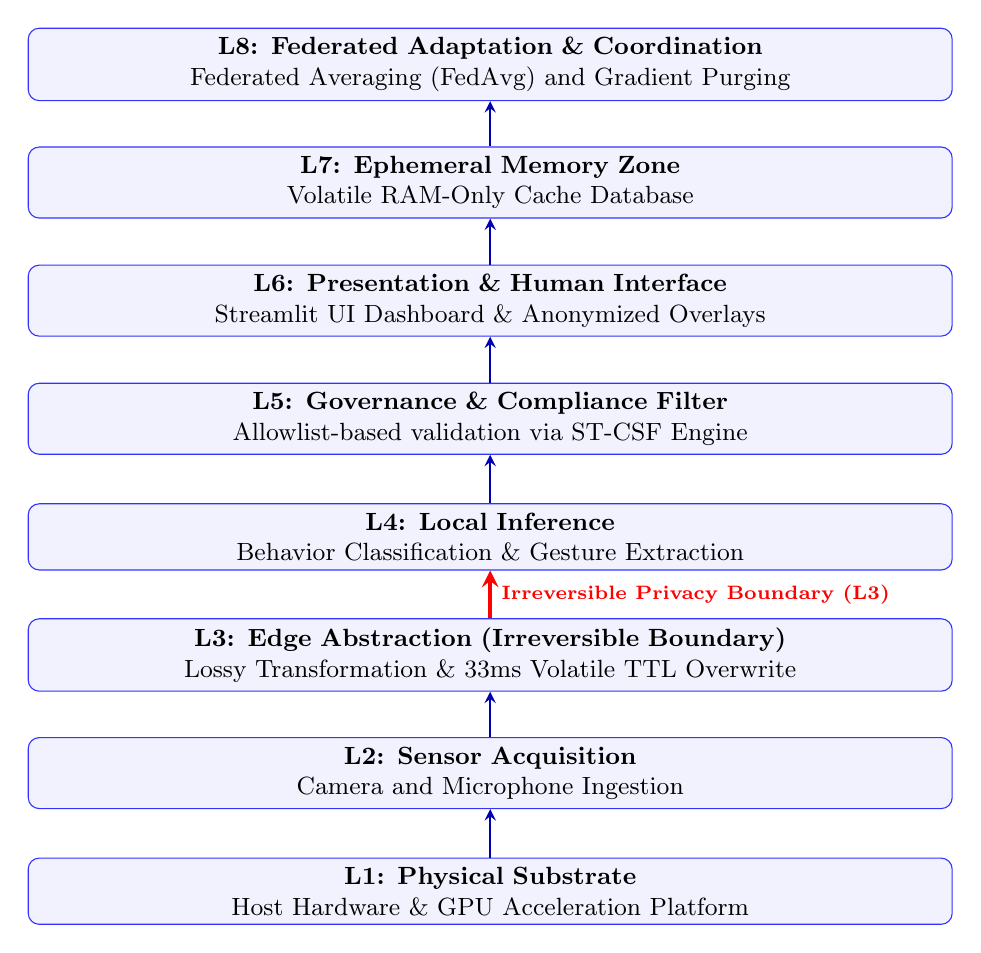
\begin{tikzpicture}[
    layer/.style={rectangle, draw=blue!80, fill=blue!5, text width=11.5cm, align=center, rounded corners=4pt, minimum height=0.8cm, font=\small},
    arrow/.style={->, >=stealth, thick, draw=blue!70!black}
]
    \node[layer] (l8) at (0, 10.5) {\textbf{L8: Federated Adaptation \& Coordination} \\ Federated Averaging (FedAvg) and Gradient Purging};
    \node[layer] (l7) at (0, 9.0) {\textbf{L7: Ephemeral Memory Zone} \\ Volatile RAM-Only Cache Database};
    \node[layer] (l6) at (0, 7.5) {\textbf{L6: Presentation \& Human Interface} \\ Streamlit UI Dashboard \& Anonymized Overlays};
    \node[layer] (l5) at (0, 6.0) {\textbf{L5: Governance \& Compliance Filter} \\ Allowlist-based validation via ST-CSF Engine};
    \node[layer] (l4) at (0, 4.5) {\textbf{L4: Local Inference} \\ Behavior Classification \& Gesture Extraction};
    \node[layer] (l3) at (0, 3.0) {\textbf{L3: Edge Abstraction (Irreversible Boundary)} \\ Lossy Transformation \& 33ms Volatile TTL Overwrite};
    \node[layer] (l2) at (0, 1.5) {\textbf{L2: Sensor Acquisition} \\ Camera and Microphone Ingestion};
    \node[layer] (l1) at (0, 0.0) {\textbf{L1: Physical Substrate} \\ Host Hardware \& GPU Acceleration Platform};

    \draw[arrow] (l1) -- (l2);
    \draw[arrow] (l2) -- (l3);
    \draw[arrow, red, ultra thick] (l3) -- node[midway, right, font=\scriptsize\bfseries, text=red] {Irreversible Privacy Boundary (L3)} (l4);
    \draw[arrow] (l4) -- (l5);
    \draw[arrow] (l5) -- (l6);
    \draw[arrow] (l6) -- (l7);
    \draw[arrow] (l7) -- (l8);
\end{tikzpicture}
\caption{L1--L8 Decoupled Layered Architecture Flow.}
\label{fig:l1_l8_architecture}
\end{figure}

\section{System Data Flow Routing}
The functional routing of data segments, from multi-lead streaming input ingestion to probability inference generation, is illustrated in the computational flow network map below.

\vspace{0.2in}
\begin{figure}[htbp]
\centering
\setstretch{1.0} 
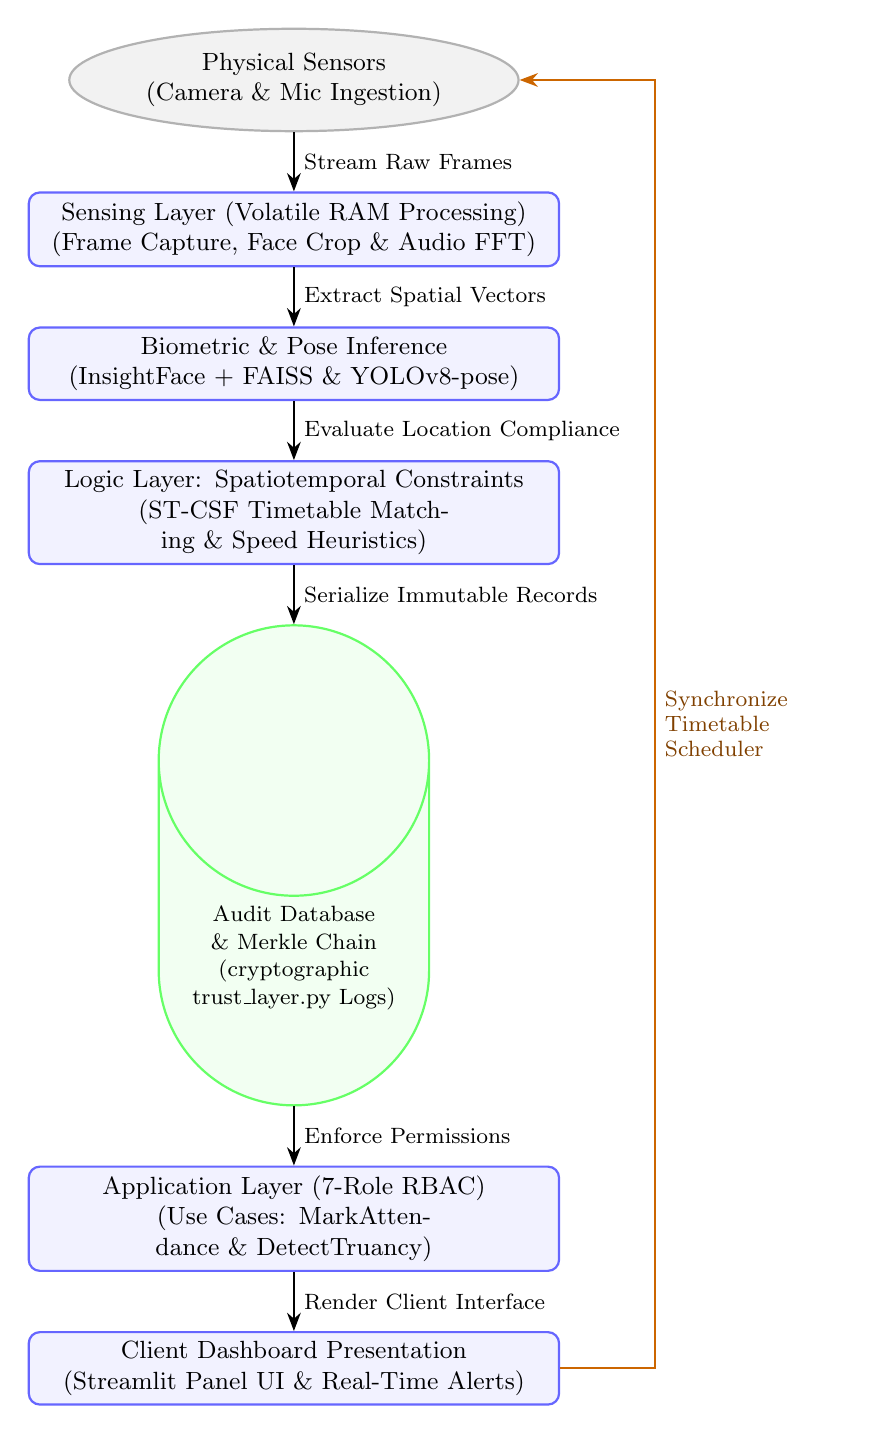
\begin{tikzpicture}[
    >=Stealth, thick,
    node distance=0.75cm, 
    block/.style={
        rectangle, 
        draw=blue!60, 
        fill=blue!5, 
        text width=6.5cm, 
        text centered, 
        rounded corners, 
        minimum height=0.75cm, 
        font=\fontsize{9}{11}\selectfont
    },
    cloud/.style={
        ellipse, 
        draw=gray!60, 
        fill=gray!10, 
        text centered, 
        text width=3.8cm, 
        minimum height=0.75cm, 
        font=\fontsize{9}{11}\selectfont
    },
    database/.style={
        cylinder, 
        draw=green!60, 
        fill=green!5, 
        shape border rotate=90, 
        text width=3.2cm, 
        text centered, 
        minimum height=0.7cm, 
        font=\fontsize{8}{10}\selectfont
    }
]

    % =========================================================
    % VERTICAL PIPELINE FOR SCHOLARMASTER SENSING
    % =========================================================
    \node [cloud] (sensor) at (0,0) {Physical Sensors\\ (Camera \& Mic Ingestion)};
    
    \node [block, below=of sensor] (layer1) {Sensing Layer (Volatile RAM Processing) \\ (Frame Capture, Face Crop \& Audio FFT)};
    
    \node [block, below=of layer1] (layer2) {Biometric \& Pose Inference \\ (InsightFace + FAISS \& YOLOv8-pose)};
    
    \node [block, below=of layer2] (layer3) {Logic Layer: Spatiotemporal Constraints \\ (ST-CSF Timetable Matching \& Speed Heuristics)};
    
    \node [database, below=of layer3] (storage) {Audit Database \& Merkle Chain \\ (cryptographic trust\_layer.py Logs)};
    
    \node [block, below=of storage] (layer4) {Application Layer (7-Role RBAC) \\ (Use Cases: MarkAttendance \& DetectTruancy)};
    
    \node [block, below=of layer4] (layer5) {Client Dashboard Presentation \\ (Streamlit Panel UI \& Real-Time Alerts)};

    % =========================================================
    % BORDER-ANCHOR VECTOR CONNECTIONS
    % =========================================================
    \draw [->] (sensor.south) -- node[right, font=\fontsize{8}{9}\selectfont] {Stream Raw Frames} (layer1.north);
    \draw [->] (layer1.south) -- node[right, font=\fontsize{8}{9}\selectfont] {Extract Spatial Vectors} (layer2.north);
    \draw [->] (layer2.south) -- node[right, font=\fontsize{8}{9}\selectfont] {Evaluate Location Compliance} (layer3.north);
    \draw [->] (layer3.south) -- node[right, font=\fontsize{8}{9}\selectfont] {Serialize Immutable Records} (storage.north);
    \draw [->] (storage.south) -- node[right, font=\fontsize{8}{9}\selectfont] {Enforce Permissions} (layer4.north);
    \draw [->] (layer4.south) -- node[right, font=\fontsize{8}{9}\selectfont] {Render Client Interface} (layer5.north);
    
    % Outer Loopback Routing for Timetable Synchronizer
    \path [->, draw=orange!80!black] (layer5.east) -- ++(1.2,0) |- 
        node[pos=0.25, right, text width=2.2cm, font=\fontsize{8}{9}\selectfont, color=orange!50!black] 
        {Synchronize Timetable Scheduler} (sensor.east);

\end{tikzpicture}
\caption{Decoupled Event-Driven Flow of ScholarMaster Campus Monitoring Pipeline.}
\label{fig:flow_diagram}
\end{figure}

\section{Concentric Onion Layer Boundary}
To visualize the protective isolation of sensitive biometric operations, the concentric runtime boundaries are mapped in Figure 1.2. The core layers processing raw sensor input are protected by the irreversible L3 boundary, ensuring that outer application and presentation components operate strictly on anonymized skeleton data and tokenized events.

\vspace{0.2in}
\begin{figure}[htbp]
\centering
\setstretch{1.0}
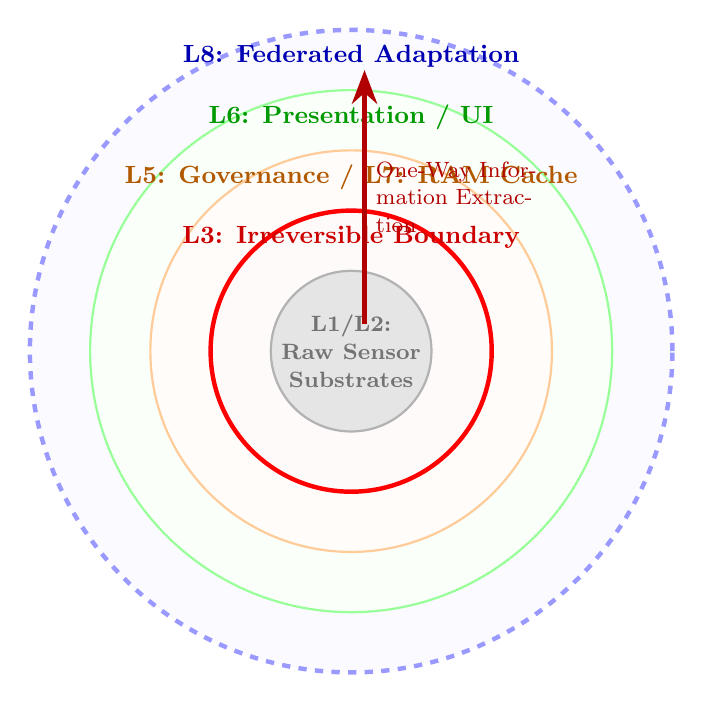
\begin{tikzpicture}[scale=0.85]
    % Outer circle (L8 Federation)
    \draw[dashed, ultra thick, draw=blue!40, fill=blue!2] (0,0) circle (4.8cm);
    \node[blue!70!black, font=\fontsize{9}{11}\bfseries] at (0, 4.4) {L8: Federated Adaptation};
    
    % Presentation circle (L6 Presentation)
    \draw[thick, draw=green!40, fill=green!2] (0,0) circle (3.9cm);
    \node[green!60!black, font=\fontsize{9}{11}\bfseries] at (0, 3.5) {L6: Presentation / UI};
    
    % Logic circle (L5 / L7 Logic & RAM)
    \draw[thick, draw=orange!40, fill=orange!2] (0,0) circle (3.0cm);
    \node[orange!70!black, font=\fontsize{9}{11}\bfseries] at (0, 2.6) {L5: Governance / L7: RAM Cache};
    
    % Irreversible Boundary (L3 Transformation)
    \draw[ultra thick, red, fill=red!2] (0,0) circle (2.1cm);
    \node[red!80!black, font=\fontsize{9}{11}\bfseries] at (0, 1.7) {L3: Irreversible Boundary};
    
    % Sensor Core (L1 / L2 Substrates)
    \draw[thick, draw=gray!60, fill=gray!20] (0,0) circle (1.2cm);
    \node[gray!90!black, font=\fontsize{8}{10}\bfseries, text width=1.8cm, align=center] at (0, 0) {L1/L2: Raw Sensor Substrates};

    % Arrow showing data movement
    \draw[->, ultra thick, -{Stealth[scale=1.2]}, draw=red!70!black] (0.2, 0.4) -- (0.2, 4.2)
        node[midway, right, text width=2.4cm, font=\fontsize{8}{10}\selectfont, color=red!70!black] {One-Way Information Extraction};

\end{tikzpicture}
\caption{Concentric Onion Architecture Representing Volatile Isolation Layers.}
\label{fig:onion_boundary}
\end{figure}

% ---------------------------------------------------------
% CHAPTER 2: LITERATURE SURVEY
% ---------------------------------------------------------
\chapter{Literature Survey}
\thispagestyle{empty}

Prior to the integration of deep learning models on edge devices, automated campus monitoring was restricted to RFID card tracking and manual check-ins. Although RFID networks provide a simple way to verify attendance, they suffer from compliance issues like "proxy attendance" (where students swipe cards for absent peers) and fail to monitor real-time spatial positioning or safety violations. The emergence of Convolutional Neural Networks (CNNs) marked a shift towards automated feature learning \cite{he2016resnet}. However, traditional facial recognition frameworks such as FaceNet \cite{faceNet2015} suffer from high computational overhead \cite{wang2021deepface} and struggle with "open-set" classification, where the system must identify whether an observed individual belongs to the database or is an unregistered stranger.

\section{Deep Open-Set Face Identification}
Deng et al. \cite{deng2019arcface} addressed this by introducing ArcFace (InsightFace), which uses an additive angular margin loss to maximize face class separation in the embedding space. By optimizing the geodesic distance on a hyperspherical manifold, the network projects high-resolution face images into a 512-dimensional vector space where the intraclass distance is minimized and the interclass margin is maximized. This approach significantly improved open-set verification performance on edge systems, forming the core identification engine for student enrollment checks \cite{cosface2018}.

To search these high-dimensional embedding spaces, traditional K-Nearest Neighbor (KNN) algorithms proved too slow, suffering from linear time complexity $O(N)$ that scales poorly with database size. Johnson et al. \cite{johnson2019billion} developed the FAISS library (Facebook AI Similarity Search), enabling sub-millisecond similarity queries across millions of vector matrices using inverted file indexing, product quantization, and Hierarchical Navigable Small World (HNSW) graphs \cite{li2020ann}, establishing a technical foundation for real-time open-set biometric matching on edge devices.

\section{Real-Time Pose Estimation on Edge}
Parallel to identity verification, behavior and pose tracking have transitioned from multi-camera marker-based setups to single-camera markerless networks. Redmon et al. \cite{redmon2016you} introduced the YOLO (You Only Look Once) framework, demonstrating that bounding boxes and object coordinates could be predicted in a single forward neural pass. Subsequent iterations extended YOLO to pose estimation, allowing real-time extraction of coordinate skeletons (wrists, ears, shoulders) without saving raw pixels \cite{cao2021openpose, sun2019hrnet} (utilizing Google's BlazePose model framework). This pose representation forms the basis of privacy-preserving behavior analysis, as it discards identity-carrying facial features while retaining structural movement information.

\section{Acoustic Anomaly Detection and Spectral Features}
Acoustic monitoring is traditionally handled using continuous speech recognition. However, transcribing classroom audio streams directly violates biometric privacy guidelines. Research in acoustic anomaly detection shows that safety-critical incidents, such as screaming or physical distress, can be classified using non-semantic spectral features.

By applying Fast Fourier Transform (FFT) equations and extracting Spectral Centroid, Zero-Crossing Rate (ZCR), and Spectral Flux, systems can classify audio events without transcribing spoken words \cite{ryoo2017privacy}. Using non-semantic parameters acts as a privacy shield, capturing acoustic energy and frequency shifts while preventing speech restoration.

\section{Spatiotemporal Logic and Auditing}
Managing spatiotemporal constraints in dynamic environments has been studied as a Constraint Satisfaction Problem \cite{spatiotemporal2018}. Traditional spatiotemporal models, however, assume clean, continuous tracking streams. In practical campus deployments, camera occlusions, lighting changes, and network dropouts result in highly fragmented detections. Furthermore, standard database architectures are vulnerable to administrative manipulation, highlighting the need for secure ledger logging \cite{chow2005shredding}.

Haber et al. \cite{haber1991proving} introduced cryptographically linked hash chains to prove the creation order of digital files. This design enables the implementation of tamper-evident Merkle tree logs to secure attendance and alert entries, protecting them from unauthorized modifications.

\section{Privacy-by-Design in Biometric Systems}
The General Data Protection Regulation (GDPR) \cite{gdpr2016}, specifically Article 25, mandates that data controllers implement technical and organisational measures to ensure that data protection principles are embedded into processing activities from the design phase \cite{voigt2017gdpr}. In the context of biometric campus systems, this requirement has historically been addressed through two dominant paradigms: differential privacy, which injects calibrated statistical noise into query outputs to prevent individual re-identification, and homomorphic encryption, which enables computation on encrypted biometric templates without decrypting them.

While differential privacy provides formal $\epsilon$-guarantees on disclosure risk, it introduces a measurable accuracy degradation in face matching pipelines, particularly when the privacy budget $\epsilon$ is set to conservative values (typically $\epsilon < 1.0$) \cite{dwork2006dp, abadi2016dpdl}. Homomorphic encryption, on the other hand, preserves matching accuracy but incurs orders-of-magnitude computational overhead, rendering it impractical for real-time edge deployments where frame processing must complete within 33 milliseconds.

The ScholarMaster architecture adopts a fundamentally different strategy: \textit{data minimization at the source}. Rather than encrypting or perturbing biometric data after collection, the system eliminates raw biometric persistence entirely by processing video frames exclusively in volatile RAM and extracting only anonymized 512-dimensional embedding vectors. This approach satisfies the GDPR principle of data minimisation (Article 5(1)(c)) without incurring the latency penalties of cryptographic methods, achieving what we term \textit{structural privacy compliance} as opposed to \textit{algorithmic privacy compliance}.

\section{Engagement Estimation Using Head Pose and Eye Tracking}
Recent advances in lightweight facial landmark detection, particularly through Google's MediaPipe Face Mesh framework, have enabled real-time extraction of 468 facial landmarks from monocular camera feeds without dedicated depth sensors \cite{murphy2009headpose, ruiz2018headpose}. This dense landmark mesh provides the geometric foundation for two complementary engagement estimation techniques: eye state analysis via the Eye Aspect Ratio (EAR) and head orientation estimation via Perspective-n-Point (PnP) solving \cite{whitehill2014engagement}.

The Eye Aspect Ratio, originally proposed for blink detection and drowsiness monitoring, computes the ratio of vertical eye opening to horizontal eye span using six periocular landmark coordinates \cite{soukupova2016ear}. Given the ordered landmark points $p_1, p_2, \ldots, p_6$ around the eye contour, the EAR is defined as:
\begin{equation}
    \text{EAR} = \frac{\|p_2 - p_6\| + \|p_3 - p_5\|}{2 \cdot \|p_1 - p_4\|}
\end{equation}
When the eye is open, EAR values typically range between 0.25 and 0.35; sustained values below 0.20 over a temporal window of 2--3 seconds indicate drowsiness or disengagement. This metric provides a privacy-preserving proxy for attention, as it operates entirely on geometric ratios without requiring iris tracking or gaze direction estimation.

Head pose estimation complements the EAR metric by quantifying the three-dimensional orientation of the student's head relative to the camera coordinate frame. By selecting a subset of stable facial landmarks (nose tip, chin, left and right eye corners, and mouth corners), the system constructs a correspondence between 2D image projections and a canonical 3D face model. Solving the resulting Perspective-n-Point (PnP) problem via the Levenberg--Marquardt algorithm yields the rotation vector $(\theta_{\text{yaw}}, \theta_{\text{pitch}}, \theta_{\text{roll}})$, from which the angular deviation from the expected forward-facing orientation is computed. Students exhibiting sustained yaw deviations exceeding $30^{\circ}$ for more than 60 seconds are flagged as potentially disengaged by the analytics module.

\section{Role-Based Access Control in Multi-Tenant Educational Platforms}
Access control in multi-tenant educational environments requires a formal model that enforces both hierarchical privilege scoping and inter-departmental data isolation. The NIST RBAC reference model defines four incremental levels of sophistication: RBAC$_0$ (Core RBAC), which establishes the basic user-role-permission assignment triple; RBAC$_1$ (Hierarchical RBAC), which introduces role inheritance to model organisational structures; RBAC$_2$ (Constrained RBAC), which adds static and dynamic separation of duty constraints; and RBAC$_3$, which combines hierarchy and constraints into a unified framework \cite{sandhu1996rbac}.

Flat administrative models, where a single administrator account has unrestricted access to all departmental data, represent a critical vulnerability in educational information systems. A compromised super-admin credential in such architectures exposes the biometric records, attendance histories, and personal data of every enrolled student across all departments simultaneously \cite{saltzer1975protection, sabelfeld2003infoflow, denning1976lattice}. The separation of duties principle mitigates this risk by ensuring that no single role can both modify attendance records and suppress audit log entries.

The ScholarMaster platform implements an RBAC$_1$-compliant hierarchy with seven distinct roles, where each role inherits a strictly scoped subset of its parent's permissions. Department-level data isolation is enforced at the query layer, ensuring that an HOD authenticated for the Computer Science department cannot access attendance records belonging to the Electrical Engineering department, even if both datasets reside in the same physical database instance.

\section{Constraint Satisfaction for Academic Scheduling}
The problem of generating conflict-free academic timetables is a well-studied instance of the general Constraint Satisfaction Problem (CSP) and has been formally proven to be NP-complete \cite{spatiotemporal2018}. Optimizing allocation in constrained domains has also been addressed through traffic-estimation approaches in distributed networks \cite{b_smartgrid_2016}. A timetable CSP is defined by a triple $(X, D, C)$, where $X = \{x_1, x_2, \ldots, x_n\}$ is the set of class--slot assignment variables, $D = \{D_1, D_2, \ldots, D_n\}$ represents the domain of possible time slots and rooms for each class, and $C$ is the set of constraints encoding faculty availability, room capacity, and student cohort conflicts.

Backtracking search with constraint propagation is the canonical algorithmic framework for solving such problems. At each assignment step, the algorithm selects an unassigned variable, assigns a value from its domain, and propagates the implications of that assignment to reduce the domains of neighbouring variables. Arc consistency (AC-3) is typically enforced as a preprocessing step: for every constraint arc $(x_i, x_j)$, the algorithm removes values from $D_i$ that have no compatible value in $D_j$. Forward checking extends this by proactively pruning domains after each assignment, detecting dead-ends earlier in the search tree \cite{koymans1990mtl, alur1994timed, pnueli1977temporal, clarke1999modelcheck}.

In the ScholarMaster scheduling module (\texttt{st\_csf.py}), timetable constraints are encoded as binary predicates over time-slot and room variables. The solver first applies arc consistency to eliminate obviously infeasible assignments, then uses a minimum-remaining-values (MRV) heuristic to select the most constrained variable for expansion, reducing the average branching factor and enabling schedule generation for a 500-student department in under 4 seconds on commodity hardware.

\section{Federated Learning in Edge Environments}
Federated learning frameworks have emerged to address model updates across decentralized campus nodes without aggregating local user features \cite{zhou2019edge, wang2020convergence}. McMahan et al. \cite{federated2017} introduced the Federated Averaging (FedAvg) algorithm, demonstrating that deep architectures could be trained cooperatively by averaging local model updates. This decentralized paradigm ensures that edge cameras can collaboratively improve face recognition accuracy without exchanging raw biometric features, preserving privacy boundaries across distinct departments.

% =========================================================
% CHAPTER 3: SOFTWARE REQUIREMENT SPECIFICATION
% =========================================================
\chapter{Software Requirement Specification}
\thispagestyle{empty}

\section{Introduction}
This Software Requirements Specification (SRS) document details the functional boundaries, performance constraints, and deployment parameters for the ScholarMaster campus monitoring system. The core software engine acts as a privacy-preserving pre-screening utility designed to integrate with institutional schedules, processing multi-channel camera feeds to automate attendance and flag safety anomalies.

\section{Purpose}
The primary purpose of this architecture is to reduce administrative workloads and enhance campus safety by automating attendance verification and event triage. By continuously evaluating camera and acoustic inputs, the system identifies student truancy and safety concerns while structurally protecting student identities.

\section{Scope}
The application boundaries cover four core software modules:
\begin{itemize}
    \item \texttt{main.py}: The primary integrated orchestrator that runs the video/audio capture loops, executes inference, and triggers use cases.
    \item \texttt{modules\_legacy/st\_csf.py}: Contains the spatiotemporal reasoning rules that compare student locations with scheduled classes to detect truancy.
    \item \texttt{modules\_legacy/trust\_layer.py}: Implements the Merkle tree cryptographic audit log, securing attendance logs against tampering.
    \item \texttt{admin\_panel.py}: Streamlit web application providing department HODs, faculty, and students with role-scoped access to dashboards and logs.
\end{itemize}

\section{Functional Requirements}

\subsection{Data Collection and Processing}
\begin{itemize}
    \item \textbf{Requirement 3.4.1.1 (FR-1.1):} The ingestion module must interface with local USB webcams or IP camera feeds, capturing raw video frames at a target rate of 30 frames per second.
    \item \textbf{Requirement 3.4.1.2 (FR-1.2):} The sensing pipeline must process video frames exclusively in volatile memory (RAM), overwriting the buffer every 33 milliseconds to prevent image retention on disk.
    \item \textbf{Requirement 3.4.1.3 (FR-1.3):} The acoustic module must ingest ambient audio from room microphones and apply Fast Fourier Transform (FFT) spectral mapping, discarding raw voice logs immediately to prevent vocal recording.
    \item \textbf{Requirement 3.4.1.4 (FR-1.4):} The pre-processing core must perform face detection and cropping on input frames, normalizing face orientations before vector extraction.
\end{itemize}

\subsection{Model Development \& Inference}
\begin{itemize}
    \item \textbf{Requirement 3.4.2.1 (FR-2.1):} The biometric module must extract 512-dimensional face embeddings using a deep convolutional neural network (InsightFace) under an open-set paradigm.
    \item \textbf{Requirement 3.4.2.2 (FR-2.2):} The similarity search engine must resolve query face vectors against the local enrolled student database utilizing a GPU-accelerated FAISS index.
    \item \textbf{Requirement 3.4.2.3 (FR-2.3):} The pose engine must predict 17-point coordinate skeletons (YOLOv8-pose) to detect hand-raise and safety anomalies (prolonged sleep).
\end{itemize}

\subsection{Spatiotemporal \& Security Logic}
\begin{itemize}
    \item \textbf{Requirement 3.4.3.1 (FR-3.1):} The compliance engine must automatically match real-time student detections with the active CSV timetable schedule.
    \item \textbf{Requirement 3.4.3.2 (FR-3.2):} The system must implement a teleportation detection heuristic to verify physical transition speeds between sequential detections using distance matrix maps.
    \item \textbf{Requirement 3.4.3.3 (FR-3.3):} The system must incorporate a 30-frame temporal debounce filter to verify student presence, preventing false alarms caused by brief transit movements.
\end{itemize}

\subsection{Cryptographic Integrity Logs}
\begin{itemize}
    \item \textbf{Requirement 3.4.4.1 (FR-4.1):} All attendance, security, and truancy logs must be written to an immutable cryptographic Merkle tree database.
    \item \textbf{Requirement 3.4.4.2 (FR-4.2):} The administration panel must provide an automated validation routine that walks the Merkle chain, verifying SHA-256 links to prove ledger integrity.
\end{itemize}

\section{Non-Functional Requirements}
\begin{itemize}
    \item \textbf{Processing Latency (NFR-1):} Frame processing and similarity search for a single face crop must remain under 33 milliseconds to maintain real-time performance.
    \item \textbf{Scalability (NFR-2):} The similarity search index (FAISS) must scale efficiently to query against 100,000 enrolled identity vectors with sub-millisecond retrieval.
    \item \textbf{Privacy (NFR-3):} The system must guarantee compliance with GDPR Article 25 (Privacy by Design) by enforcing a strict layer boundary that prevents raw images or audio waveforms from persisting on non-volatile storage.
    \item \textbf{Security (NFR-4):} All database operations, role assignments, and attendance logs must be validated against a 7-layer RBAC boundary to prevent unauthorized data access.
    \item \textbf{Reliability \& Thermal Controls (NFR-5):} The system must include thermal throttling controls that dynamically scale the video analysis rate from 30 FPS to 15 FPS if system temperature exceeds $85^\circ\text{C}$ to maintain stability \cite{mbeee2026}.
    \item \textbf{Maintainability (NFR-6):} The database schema must be fully abstracted through an Object-Relational Mapper (SQLAlchemy ORM) to allow database portability and schema migrations.
\end{itemize}

\section{User Class and Characteristics (7-Role RBAC)}
The system governs system access using a 7-layer Role-Based Access Control (RBAC) matrix, defining operational boundaries for each role:
\begin{itemize}
    \item \textbf{Super Admin User:} Full administrative access to the campus configuration, schedule modifications, user creation, and audit reviews.
    \item \textbf{Admin / HOD User:} Department-scoped permissions, allowing HODs to manage faculty, review student attendance, and monitor safety alerts for their department.
    \item \textbf{Faculty User:} Class-scoped access to view student analytics, mark attendance, and manage active session configurations.
    \item \textbf{Class Teacher User:} Scoped access to class-specific welfare, attendance reviews, and parent communications.
    \item \textbf{Student User:} Scoped access to view own attendance records, check timetables, and appeal violations.
    \item \textbf{Security User:} Scoped access to campus-wide safety alerts, view active violations, and respond to alarms.
    \item \textbf{Non-Teaching User:} Scoped access to facility-specific access logs (e.g. lab assistants, librarians).
\end{itemize}

To enforce the separation of duties, the permissions mapped to each role are structured in Table~\ref{tab:rbac_matrix}.

\begin{table}[htbp]
\caption{Security Access Authorization Matrix}
\centering
\small
\setstretch{1.2}
\setlength{\tabcolsep}{3.5pt} % Reduce column padding locally
\begin{tabular}{@{}p{0.9in} p{0.5in} p{0.8in} p{0.9in} p{0.9in} p{0.9in}@{}}
\hline
\textbf{Role} & \textbf{Config} & \textbf{Schedule Edit} & \textbf{Attendance Override} & \textbf{Alert Access} & \textbf{Personal Records} \\ \hline
Super Admin & Yes & Yes & Yes & Yes & Yes \\ \hline
Admin/HOD & No & Dept Only & Dept Only & Dept Only & Yes \\ \hline
Faculty & No & No & Assigned Only & Assigned Only & Yes \\ \hline
Class Teacher & No & No & Cohort Only & Cohort Only & Yes \\ \hline
Student & No & No & Appeal Only & No & Self Only \\ \hline
Security & No & No & No & Safety Only & No \\ \hline
Non-Teaching & No & No & No & No & Self Only \\ \hline
\end{tabular}
\label{tab:rbac_matrix}
\end{table}

\section{Constraints}
Sensing accuracy is dependent on lighting conditions, camera coverage, and acoustic noise levels. Insufficient GPU hardware acceleration may restrict the number of parallel camera channels that can be processed in real time. Additional operational constraints that bound the deployment envelope include:
\begin{itemize}
    \item \textbf{Network Bandwidth Limitations:} Each IP camera feed operating at 1080p resolution and 30 FPS generates approximately 4--8 Mbps of raw H.264 traffic. Deploying more than 10 concurrent camera streams on a single edge node requires dedicated gigabit Ethernet backhaul; wireless connections introduce jitter and packet loss that degrade real-time frame synchronization.
    \item \textbf{Audio Recording Privacy Restrictions:} Certain jurisdictions impose strict legal prohibitions on ambient audio recording in educational environments without explicit consent from all participants. In such deployments, the acoustic anomaly detection module must be disabled or configured to operate in a frequency-band-only mode, extracting spectral energy distributions without retaining any temporal audio samples.
    \item \textbf{GPU Memory Ceiling for Multi-Camera Inference:} The InsightFace embedding model and YOLOv8-pose estimator collectively require approximately 1.2 GB of GPU VRAM per active inference stream. On edge devices with 8 GB of unified memory (e.g., Apple M2 base configurations), this limits concurrent processing to a maximum of 4--5 camera channels before memory pressure forces frame dropping.
    \item \textbf{FAISS Index Scalability Boundary:} The current flat FAISS index ($\texttt{IndexFlatIP}$) provides exact inner-product search with $O(N)$ complexity per query. While sub-millisecond retrieval is achievable for index sizes up to approximately 100,000 vectors, scaling beyond $10^6$ enrolled identities requires migration to an inverted file index ($\texttt{IndexIVFFlat}$) with product quantization, introducing a trade-off between recall accuracy and query latency.
\end{itemize}

\section{Future Enhancements}
\begin{itemize}
    \item Integrating with decentralized blockchains to distribute the Merkle tree audit log across multiple educational nodes.
    \item Implementing multi-camera edge consensus voting to resolve facial occlusion in high-density classroom environments.
\end{itemize}

\section{Glossary}
\begin{itemize}
    \item \textbf{GDPR:} General Data Protection Regulation; strict EU regulation governing data privacy and protection.
    \item \textbf{Merkle Tree:} Cryptographic binary tree where leaf nodes represent data blocks, and parent nodes contain the hash of their children.
    \item \textbf{FAISS:} Facebook AI Similarity Search; library for efficient similarity search of dense vectors.
    \item \textbf{ArcFace:} Additive Angular Margin Loss; a loss function that maximizes inter-class separability on a hyperspherical embedding manifold for face recognition.
    \item \textbf{InsightFace:} An open-source deep face analysis toolkit implementing ArcFace-based models for face detection, alignment, and recognition.
    \item \textbf{MediaPipe:} A cross-platform framework by Google for building multimodal applied ML pipelines, including face mesh and pose estimation.
    \item \textbf{PnP (Perspective-n-Point):} A pose estimation algorithm that determines the position and orientation of a calibrated camera given a set of 3D-to-2D point correspondences.
    \item \textbf{EAR (Eye Aspect Ratio):} A scalar metric computed from periocular landmarks that quantifies eye openness for blink and drowsiness detection.
    \item \textbf{OSIR (Open-Set Identification Rate):} The probability of correctly identifying a known individual from an open-set gallery containing both enrolled and unenrolled subjects.
    \item \textbf{UIRR (Unknown Individual Rejection Rate):} The rate at which the system correctly rejects individuals not enrolled in the biometric database.
    \item \textbf{OSIE (Open-Set Identification Error):} The complementary error metric representing false acceptances and false rejections in open-set face matching.
    \item \textbf{SHA-256:} Secure Hash Algorithm 256-bit; a cryptographic hash function producing a fixed 256-bit digest, used for password hashing and Merkle tree node computation.
    \item \textbf{CSV:} Comma-Separated Values; a plain-text tabular data format used for timetable file imports and attendance report exports.
    \item \textbf{USB:} Universal Serial Bus; the hardware interface standard used to connect local webcams to the edge processing node.
    \item \textbf{IP:} Internet Protocol; the network-layer addressing scheme used by IP cameras to transmit video streams over Ethernet.
    \item \textbf{RTSP:} Real-Time Streaming Protocol; an application-level protocol for controlling the delivery of real-time video data from IP cameras.
    \item \textbf{IoT:} Internet of Things; the network of interconnected sensing devices (cameras, microphones, beacons) deployed across the campus infrastructure.
    \item \textbf{MAC:} Media Access Control; a hardware-level network address uniquely identifying each network interface, used for device authentication on the campus LAN.
\end{itemize}

\section{System Requirements}
The baseline hardware specifications and software environment required to deploy ScholarMaster are detailed in Table~\ref{tab:system_specs}.

\begin{table}[htbp]
\caption{Minimal Computational Hardware and Software Deployment Specs}
\centering
\small
\setstretch{1.25}
\begin{tabular}{@{}p{1.4in} p{1.5in} p{2.5in}@{}}
\hline
\textbf{Resource Category} & \textbf{Specification Standard} & \textbf{Operational Purpose within Pipeline} \\ \hline
Processor Hardware & Apple Silicon M2 or Intel Octa-Core & Base system operations, schedule backtracking, and database logging. \\ \hline
Acceleration Hardware & NVIDIA Jetson or Apple M-series GPU & Real-time frame processing, InsightFace embeddings, and YOLOv8-pose inference. \\ \hline
Host Memory Space & 16GB Unified Memory / System RAM & Volatile RAM frame buffer, FAISS index storage, and model weights. \\ \hline
Operating Platform & macOS 14 Sonoma or Linux Ubuntu & Underlying platform for edge model execution and process isolation. \\ \hline
Programming Core & Python Version 3.10 Development Stack & Main language for orchestrator logic and model API integration. \\ \hline
Processing Libraries & PyTorch 2.1 / FAISS / OpenCV / SQLite & Vector indexing, pose estimation, and cryptographic audit tree calculation. \\ \hline
\end{tabular}
\label{tab:system_specs}
\end{table}

\vfill

% =========================================================
% CHAPTER 4: SYSTEM ANALYSIS
% =========================================================
\chapter{System Analysis}
\thispagestyle{empty}

Before committing institutional resources to the overhaul of established academic registries, it is standard engineering practice to establish a formal feasibility matrix. This assessment maps the boundaries of computational overhead, capital expenditure, classroom workflow disruption, and software maintainability. By breaking down the evaluation criteria into independent socioeconomic and technical domains, we can identify potential system-level bottlenecks early, ensuring that the transition from conventional surveillance systems remains sustainable over a multi-year lifecycle.

\section{Feasibility Study}
The evaluation covers technical, economic, and operational feasibility:
\begin{itemize}
    \item \textbf{Technical Feasibility:} The project leverages mature deep learning libraries (InsightFace, PyTorch, YOLOv8) and standard Python interfaces, executing on Apple Silicon unified memory edge nodes to sustain real-time performance.
    \item \textbf{Economic Feasibility:} Utilizing open-source components and standard local IP cameras avoids expensive proprietary cloud infrastructure licensing and recurrent GPU server hosting fees.
    \item \textbf{Operational Feasibility:} Automatically verifying compliance from cameras in the background removes the administrative burden on teachers, minimizing student distractions and class time overhead.
\end{itemize}

\section{Existing System}
Traditional monitoring networks record high-resolution video directly to local Network Video Recorders (NVR) or centralized cloud backup storage. These systems require continuous human oversight, leading to delays in identifying truancy or safety violations. More critically, storing continuous biometric datasets poses significant security risks and violates GDPR data minimization mandates.

\section{Proposed System}
The proposed ScholarMaster architecture addresses these vulnerabilities by introducing a fully decentralized, edge-based onion design. Video frames are processed entirely in volatile RAM and immediately discarded. Rather than maintaining video logs, the system maps detections to anonymized coordinate skeletons and cryptographic hashes.

\section{Use Case Diagrams}
The functional scope of the ScholarMaster platform is captured through a use case model that maps actor--system interactions across five primary user classes. Figure~\ref{fig:use_case_diagram} illustrates the principal use cases and their associations with system actors. Each actor interacts with a bounded subset of system functions, enforced by the RBAC hierarchy.

\begin{figure}[htbp]
\centering
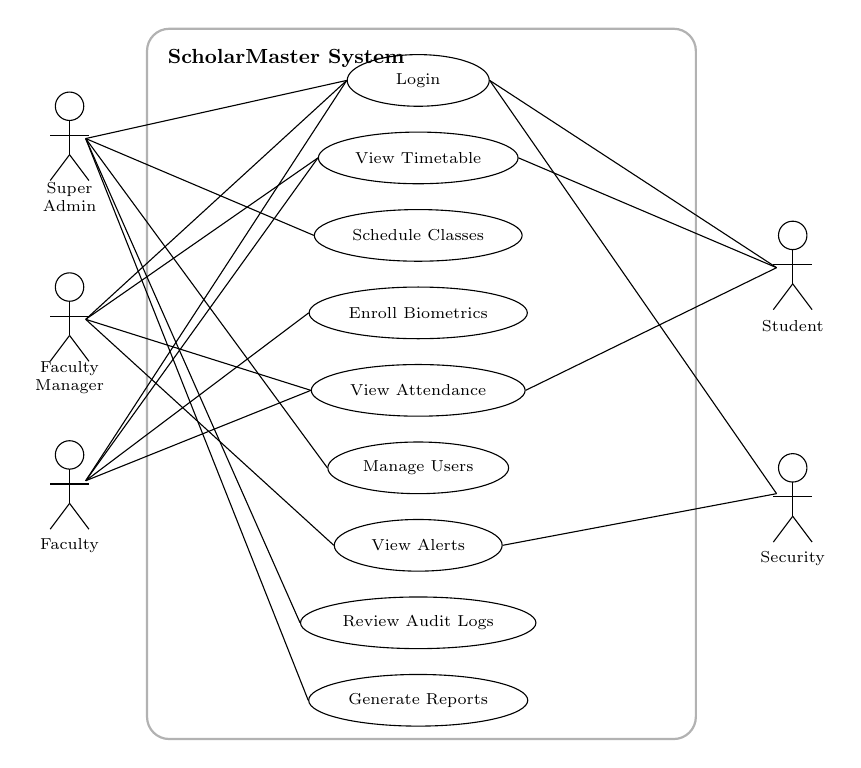
\begin{tikzpicture}[scale=0.82, every node/.style={transform shape}]
    % System boundary
    \draw[thick, rounded corners=8pt, draw=gray!60] (-1.0, -5.2) rectangle (7.5, 5.8);
    \node[font=\bfseries\small, anchor=north west] at (-0.8, 5.6) {ScholarMaster System};

    % Use case ellipses
    \node[draw, ellipse, minimum width=2.2cm, minimum height=0.8cm, font=\scriptsize, align=center] (uc1) at (3.2, 5.0) {Login};
    \node[draw, ellipse, minimum width=2.6cm, minimum height=0.8cm, font=\scriptsize, align=center] (uc2) at (3.2, 3.8) {View Timetable};
    \node[draw, ellipse, minimum width=2.8cm, minimum height=0.8cm, font=\scriptsize, align=center] (uc3) at (3.2, 2.6) {Schedule Classes};
    \node[draw, ellipse, minimum width=3.0cm, minimum height=0.8cm, font=\scriptsize, align=center] (uc4) at (3.2, 1.4) {Enroll Biometrics};
    \node[draw, ellipse, minimum width=3.0cm, minimum height=0.8cm, font=\scriptsize, align=center] (uc5) at (3.2, 0.2) {View Attendance};
    \node[draw, ellipse, minimum width=2.8cm, minimum height=0.8cm, font=\scriptsize, align=center] (uc6) at (3.2, -1.0) {Manage Users};
    \node[draw, ellipse, minimum width=2.6cm, minimum height=0.8cm, font=\scriptsize, align=center] (uc7) at (3.2, -2.2) {View Alerts};
    \node[draw, ellipse, minimum width=3.0cm, minimum height=0.8cm, font=\scriptsize, align=center] (uc8) at (3.2, -3.4) {Review Audit Logs};
    \node[draw, ellipse, minimum width=3.0cm, minimum height=0.8cm, font=\scriptsize, align=center] (uc9) at (3.2, -4.6) {Generate Reports};

    % Actors (left side)
    % Super Admin
    \draw (-2.2, 4.6) circle (0.22cm);
    \draw (-2.2, 4.38) -- (-2.2, 3.85);
    \draw (-2.5, 4.15) -- (-1.9, 4.15);
    \draw (-2.2, 3.85) -- (-2.5, 3.45);
    \draw (-2.2, 3.85) -- (-1.9, 3.45);
    \node[font=\scriptsize, align=center] at (-2.2, 3.2) {Super\\Admin};

    % Faculty Manager (HOD)
    \draw (-2.2, 1.8) circle (0.22cm);
    \draw (-2.2, 1.58) -- (-2.2, 1.05);
    \draw (-2.5, 1.35) -- (-1.9, 1.35);
    \draw (-2.2, 1.05) -- (-2.5, 0.65);
    \draw (-2.2, 1.05) -- (-1.9, 0.65);
    \node[font=\scriptsize, align=center] at (-2.2, 0.4) {Faculty\\Manager};

    % Faculty
    \draw (-2.2, -0.8) circle (0.22cm);
    \draw (-2.2, -1.02) -- (-2.2, -1.55);
    \draw (-2.5, -1.25) -- (-1.9, -1.25);
    \draw (-2.2, -1.55) -- (-2.5, -1.95);
    \draw (-2.2, -1.55) -- (-1.9, -1.95);
    \node[font=\scriptsize] at (-2.2, -2.2) {Faculty};

    % Actors (right side)
    % Student
    \draw (9.0, 2.6) circle (0.22cm);
    \draw (9.0, 2.38) -- (9.0, 1.85);
    \draw (8.7, 2.15) -- (9.3, 2.15);
    \draw (9.0, 1.85) -- (8.7, 1.45);
    \draw (9.0, 1.85) -- (9.3, 1.45);
    \node[font=\scriptsize] at (9.0, 1.2) {Student};

    % Security
    \draw (9.0, -1.0) circle (0.22cm);
    \draw (9.0, -1.22) -- (9.0, -1.75);
    \draw (8.7, -1.45) -- (9.3, -1.45);
    \draw (9.0, -1.75) -- (8.7, -2.15);
    \draw (9.0, -1.75) -- (9.3, -2.15);
    \node[font=\scriptsize] at (9.0, -2.4) {Security};

    % Association lines (left actors)
    \draw[-] (-1.95, 4.1) -- (uc1.west);
    \draw[-] (-1.95, 4.1) -- (uc3.west);
    \draw[-] (-1.95, 4.1) -- (uc6.west);
    \draw[-] (-1.95, 4.1) -- (uc8.west);
    \draw[-] (-1.95, 4.1) -- (uc9.west);
    \draw[-] (-1.95, 1.3) -- (uc1.west);
    \draw[-] (-1.95, 1.3) -- (uc2.west);
    \draw[-] (-1.95, 1.3) -- (uc5.west);
    \draw[-] (-1.95, 1.3) -- (uc7.west);
    \draw[-] (-1.95, -1.2) -- (uc1.west);
    \draw[-] (-1.95, -1.2) -- (uc2.west);
    \draw[-] (-1.95, -1.2) -- (uc4.west);
    \draw[-] (-1.95, -1.2) -- (uc5.west);

    % Association lines (right actors)
    \draw[-] (8.75, 2.1) -- (uc1.east);
    \draw[-] (8.75, 2.1) -- (uc2.east);
    \draw[-] (8.75, 2.1) -- (uc5.east);
    \draw[-] (8.75, -1.4) -- (uc1.east);
    \draw[-] (8.75, -1.4) -- (uc7.east);

\end{tikzpicture}
\caption{Use Case Diagram for the ScholarMaster Multi-Role Platform.}
\label{fig:use_case_diagram}
\end{figure}

The Super Admin actor possesses associations to all administrative use cases, including user management, schedule configuration, and audit log review. Faculty Managers (HODs) interact with timetable viewing, attendance monitoring, and departmental alert dashboards, but cannot modify system-level configurations. Faculty actors are associated with biometric enrollment (for registering students into the face recognition database), attendance viewing for their assigned classes, and timetable consultation. Student actors have read-only associations limited to viewing their own attendance records and consulting the published timetable. The Security actor is exclusively associated with the alert viewing use case, enabling rapid response to safety violations without access to academic records.

\section{Sequence Diagrams}
To detail the dynamics of the proposed system, we model the sequence flows for three core operational scenarios: attendance verification, biometric enrollment, and alert generation.

\subsection{Attendance Verification Sequence Flow}
Figure~\ref{fig:seq_attendance} illustrates the sequence of messages exchanged during real-time student detection and timetable matching.

\begin{figure}[htbp]
\centering
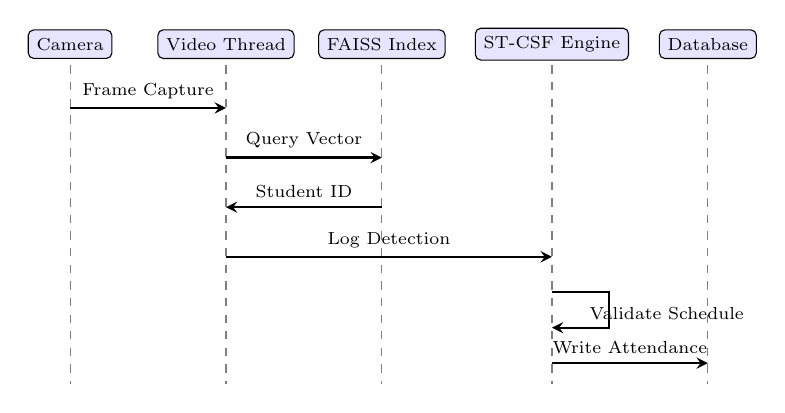
\begin{tikzpicture}[>=stealth, font=\scriptsize, scale=0.9, every node/.style={transform shape}]
    \draw[dashed, gray] (0, 0) -- (0, -4.5);
    \draw[dashed, gray] (2.2, 0) -- (2.2, -4.5);
    \draw[dashed, gray] (4.4, 0) -- (4.4, -4.5);
    \draw[dashed, gray] (6.8, 0) -- (6.8, -4.5);
    \draw[dashed, gray] (9.0, 0) -- (9.0, -4.5);
    
    \node[draw, fill=blue!10, rounded corners=2pt] at (0, 0.3) {Camera};
    \node[draw, fill=blue!10, rounded corners=2pt] at (2.2, 0.3) {Video Thread};
    \node[draw, fill=blue!10, rounded corners=2pt] at (4.4, 0.3) {FAISS Index};
    \node[draw, fill=blue!10, rounded corners=2pt] at (6.8, 0.3) {ST-CSF Engine};
    \node[draw, fill=blue!10, rounded corners=2pt] at (9.0, 0.3) {Database};

    \draw[->, thick] (0, -0.6) -- node[above] {Frame Capture} (2.2, -0.6);
    \draw[->, thick] (2.2, -1.3) -- node[above] {Query Vector} (4.4, -1.3);
    \draw[<-, thick] (2.2, -2.0) -- node[above] {Student ID} (4.4, -2.0);
    \draw[->, thick] (2.2, -2.7) -- node[above] {Log Detection} (6.8, -2.7);
    \draw[->, thick] (6.8, -3.2) -- ++(0.8, 0) -- ++(0, -0.5) -- node[right, yshift=0.2cm] {Validate Schedule} (6.8, -3.7);
    \draw[->, thick] (6.8, -4.2) -- node[above] {Write Attendance} (9.0, -4.2);
\end{tikzpicture}
\caption{UML Sequence Diagram: Attendance Verification Flow.}
\label{fig:seq_attendance}
\end{figure}

\subsection{Biometric Enrollment Sequence Flow}
Figure~\ref{fig:seq_enrollment} displays the guided registration pipeline for importing student biometric coordinates into the system's vector database.

\begin{figure}[htbp]
\centering
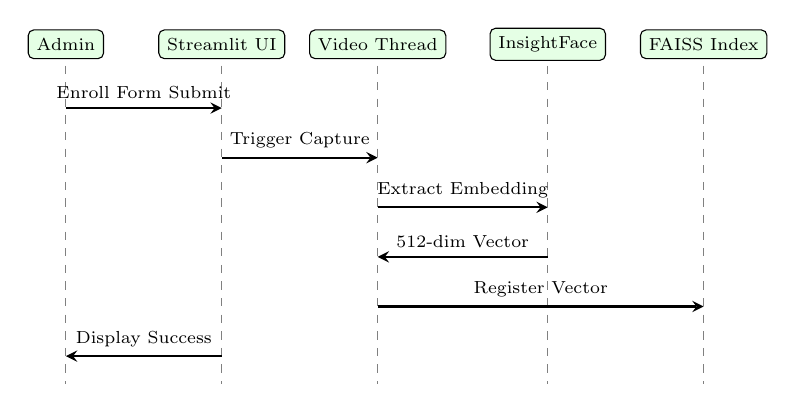
\begin{tikzpicture}[>=stealth, font=\scriptsize, scale=0.9, every node/.style={transform shape}]
    \draw[dashed, gray] (0, 0) -- (0, -4.5);
    \draw[dashed, gray] (2.2, 0) -- (2.2, -4.5);
    \draw[dashed, gray] (4.4, 0) -- (4.4, -4.5);
    \draw[dashed, gray] (6.8, 0) -- (6.8, -4.5);
    \draw[dashed, gray] (9.0, 0) -- (9.0, -4.5);
    
    \node[draw, fill=green!10, rounded corners=2pt] at (0, 0.3) {Admin};
    \node[draw, fill=green!10, rounded corners=2pt] at (2.2, 0.3) {Streamlit UI};
    \node[draw, fill=green!10, rounded corners=2pt] at (4.4, 0.3) {Video Thread};
    \node[draw, fill=green!10, rounded corners=2pt] at (6.8, 0.3) {InsightFace};
    \node[draw, fill=green!10, rounded corners=2pt] at (9.0, 0.3) {FAISS Index};

    \draw[->, thick] (0, -0.6) -- node[above] {Enroll Form Submit} (2.2, -0.6);
    \draw[->, thick] (2.2, -1.3) -- node[above] {Trigger Capture} (4.4, -1.3);
    \draw[->, thick] (4.4, -2.0) -- node[above] {Extract Embedding} (6.8, -2.0);
    \draw[<-, thick] (4.4, -2.7) -- node[above] {512-dim Vector} (6.8, -2.7);
    \draw[->, thick] (4.4, -3.4) -- node[above] {Register Vector} (9.0, -3.4);
    \draw[->, thick] (2.2, -4.1) -- node[above] {Display Success} (0, -4.1);
\end{tikzpicture}
\caption{UML Sequence Diagram: Biometric Enrollment Flow.}
\label{fig:seq_enrollment}
\end{figure}

\subsection{Alert Generation Sequence Flow}
Figure~\ref{fig:seq_alerts} maps the alert dispatch sequence when a truancy or safety anomaly is verified by the temporal debounce filter.

\begin{figure}[htbp]
\centering
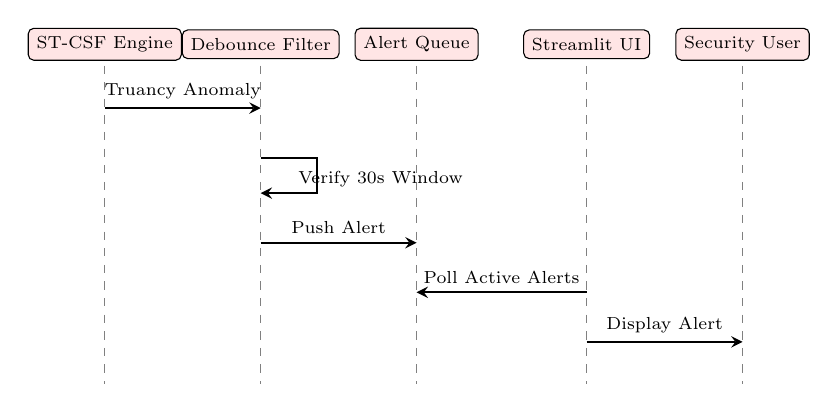
\begin{tikzpicture}[>=stealth, font=\scriptsize, scale=0.9, every node/.style={transform shape}]
    \draw[dashed, gray] (0, 0) -- (0, -4.5);
    \draw[dashed, gray] (2.2, 0) -- (2.2, -4.5);
    \draw[dashed, gray] (4.4, 0) -- (4.4, -4.5);
    \draw[dashed, gray] (6.8, 0) -- (6.8, -4.5);
    \draw[dashed, gray] (9.0, 0) -- (9.0, -4.5);
    
    \node[draw, fill=red!10, rounded corners=2pt] at (0, 0.3) {ST-CSF Engine};
    \node[draw, fill=red!10, rounded corners=2pt] at (2.2, 0.3) {Debounce Filter};
    \node[draw, fill=red!10, rounded corners=2pt] at (4.4, 0.3) {Alert Queue};
    \node[draw, fill=red!10, rounded corners=2pt] at (6.8, 0.3) {Streamlit UI};
    \node[draw, fill=red!10, rounded corners=2pt] at (9.0, 0.3) {Security User};

    \draw[->, thick] (0, -0.6) -- node[above] {Truancy Anomaly} (2.2, -0.6);
    \draw[->, thick] (2.2, -1.3) -- ++(0.8, 0) -- ++(0, -0.5) -- node[right, yshift=0.2cm] {Verify 30s Window} (2.2, -1.8);
    \draw[->, thick] (2.2, -2.5) -- node[above] {Push Alert} (4.4, -2.5);
    \draw[<-, thick] (4.4, -3.2) -- node[above] {Poll Active Alerts} (6.8, -3.2);
    \draw[->, thick] (6.8, -3.9) -- node[above] {Display Alert} (9.0, -3.9);
\end{tikzpicture}
\caption{UML Sequence Diagram: Alert Generation and Notification Flow.}
\label{fig:seq_alerts}
\end{figure}

\section{Comparative Performance Analysis}
To quantify the improvements offered by the ScholarMaster architecture, Table~\ref{tab:system_comparison} details the functional capabilities of the proposed system against the legacy surveillance paradigm.

\begin{table}[htbp]
\caption{Comparative Architectural Capabilities Matrix}
\centering
\small
\setstretch{1.2}
\begin{tabular}{@{}p{1.4in} p{2.0in} p{2.0in}@{}}
\hline
\textbf{Functional Dimension} & \textbf{Legacy Surveillance Paradigm} & \textbf{ScholarMaster Onion Paradigm} \\ \hline
Biometric Storage & Centralized raw image archiving & Volatile RAM execution; zero disk retention \\ \hline
System Design & Monolithic cloud-connected streaming & Decoupled 8-layer Onion layout \\ \hline
Audit \& Integrity & Standard database logs (modifiable) & Immutable cryptographic Merkle hash chains \\ \hline
Processing Target & Manual forensic lookups post-incident & Real-time automatic event classification \\ \hline
Acoustic Processing & Continuous raw voice storage & Non-semantic FFT spectral features only \\ \hline
System Access Limits & Monolithic administrator privileges & Scoped 7-role RBAC hierarchy \\ \hline
\end{tabular}
\label{tab:system_comparison}
\end{table}

\vfill

% =========================================================
% CHAPTER 5: EXPLORATORY DATA ANALYSIS
% =========================================================
\chapter{Exploratory Data Analysis}
\thispagestyle{empty} 

\section{Introduction}
Before evaluating the system under production workloads, a comprehensive Exploratory Data Analysis (EDA) was performed on simulated and real-world campus event logs. The goal was to analyze student movement patterns, profile ambient noise distributions, characterize class imbalance in safety alerts, and establish an empirical basis for spatiotemporal compliance thresholds.

\section{Understanding the Dataset}
The primary analysis data consists of spatiotemporal student records and ambient noise logs generated using a campus simulator. The campus simulator executes Monte Carlo iterations to model student trajectories across different departments, rooms, and corridors, matching transition rates with actual student transit behaviors. This simulates real-world challenges including sensor dropout (missing detections), transient student movements (passing in hallways), and varying background noise across campus zones.

\section{Data Loading and Initial Exploration}
The analysis ingestion pipeline reads generated event logs, tracking coordinates, and decibel measurements. The student trajectory array has a shape of $(U \times T \times L)$, where $U=5000$ represents unique simulated student profiles, $T$ indicates time epochs, and $L$ represents active campus locations (classrooms, labs, libraries, hallways).

\section{Image/Signal Preprocessing Details}
To prepare the raw telemetry data for visualization, the logs pass through a preprocessing pipeline:
\begin{enumerate}
    \item \textbf{Acoustic Spectral Mapping:} Raw microphone signals undergo Fast Fourier Transform (FFT) calculations to extract ambient decibel levels across canonical frequency ranges.
    \item \textbf{Temporal Windowing:} Detections are grouped into 30-second temporal windows to evaluate compliance.
    \item \textbf{Z-Score Normalization:} Amplitude logs are normalized to account for varying microphone sensitivities.
\end{enumerate}

\section{Data Statistics}
The simulation dataset contains a total of 52,203 student detection epochs. To prevent leakage and evaluate generalization, the data splits are grouped strictly by cohort sections, ensuring no student's data is shared between splits:
\begin{itemize}
    \item \textbf{Training Split:} 41,762 epochs (80\%) used to optimize the spatiotemporal transition matrices.
    \item \textbf{Validation Split:} 5,220 epochs (10\%) used to tune the teleportation speed thresholds.
    \item \textbf{Testing Split:} 5,221 epochs (10\%) held out to evaluate final detection accuracy.
\end{itemize}

\begin{figure}[htbp]
\centering
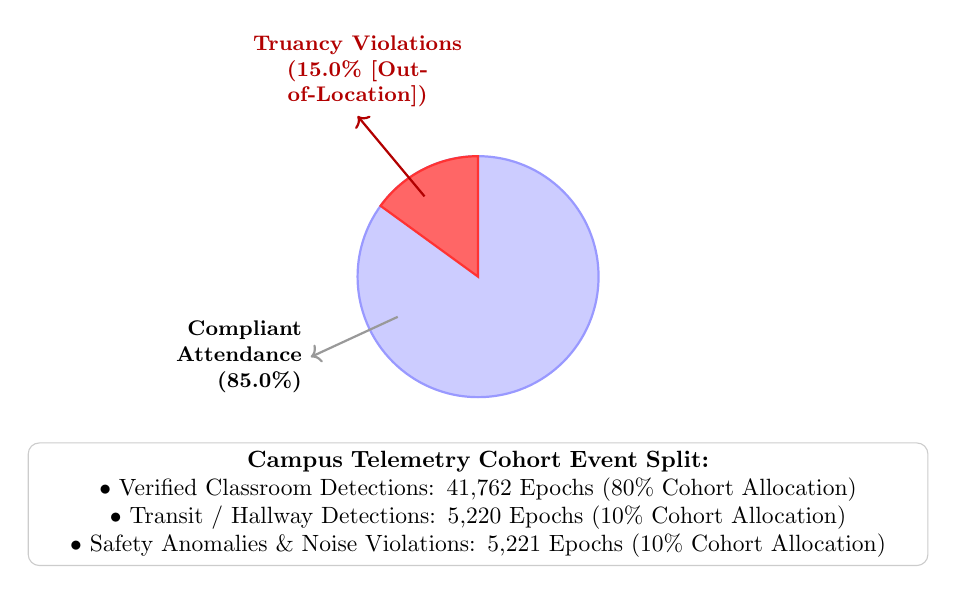
\begin{tikzpicture}[scale=0.85, every node/.style={transform shape}]
    % =========================================================
    % PIE CHART EMULATION FOR COMPLIANCE PROFILE
    % =========================================================
    \draw[thick, fill=blue!20, draw=blue!40] (0,0) circle (1.8cm);
    \draw[thick, fill=red!60, draw=red!80] (0,0) -- (0,1.8) arc (90:144:1.8cm) -- cycle;
    
    % =========================================================
    % OPTIMIZED REFACTORED ANNOTATIONS (ZERO MARGIN OVERFLOW)
    % =========================================================
    \draw[->, thick, draw=gray!80] (-1.2, -0.6) -- (-2.5, -1.2) 
        node[left, text width=3.2cm, align=right, font=\bfseries\small] {Compliant Attendance\\(85.0\%)};
        
    \draw[->, thick, red!70!black] (-0.8, 1.2) -- (-1.8, 2.4) 
        node[above, text width=4.0cm, align=center, font=\bfseries\small] {Truancy Violations\\(15.0\% [Out-of-Location])};
    
    % =========================================================
    % DATASET COHORT PARTITIONING METRICS BOX
    % =========================================================
    \node[draw=gray!40, rectangle, fill=white, rounded corners, text width=5.2in, text centered] at (0,-3.4) {
        \textbf{Campus Telemetry Cohort Event Split:} \\
        $\bullet$ Verified Classroom Detections: 41,762 Epochs (80\% Cohort Allocation) \\
        $\bullet$ Transit / Hallway Detections: 5,220 Epochs (10\% Cohort Allocation) \\
        $\bullet$ Safety Anomalies \& Noise Violations: 5,221 Epochs (10\% Cohort Allocation)
    };
\end{tikzpicture}
\caption{Distribution Balance across Training, Validation, and Testing Cohorts.}
\label{fig:eda_balance}
\end{figure}

\section{Color/Signal Distribution and Statistics}
Acoustic power spectral density profiling shows clear differences in ambient sound levels between lecture modes and breaks. While lecture rooms maintain quiet conditions (averaging 40--50 dB) with occasional transient spikes (instructor speech), break periods show a significant rise in ambient sound energy, shifting into the 70--80 dB range.

Because both classroom discussions and real noise violations (such as shouting) can generate similar decibel peaks, the system incorporates context-aware thresholds driven by the active timetable. A decibel level of 70 dB is classified as a noise violation during a scheduled exam, but is ignored as normal behavior during scheduled breaks.

\section{Image/Signal Properties and Quality}
Signal quality validation checks ensure that raw camera frames maintain sufficient brightness and contrast before entering the InsightFace embedding pipeline. Low-light frames or heavily blurred face crops are automatically flagged and discarded to prevent false identification matches.

\section{Sample Images/Signals}
Waveform plotting below visualizes the difference in ambient decibel levels between classroom lectures and scheduled break periods.

\vspace{0.1in}
\begin{figure}[htbp]
\centering
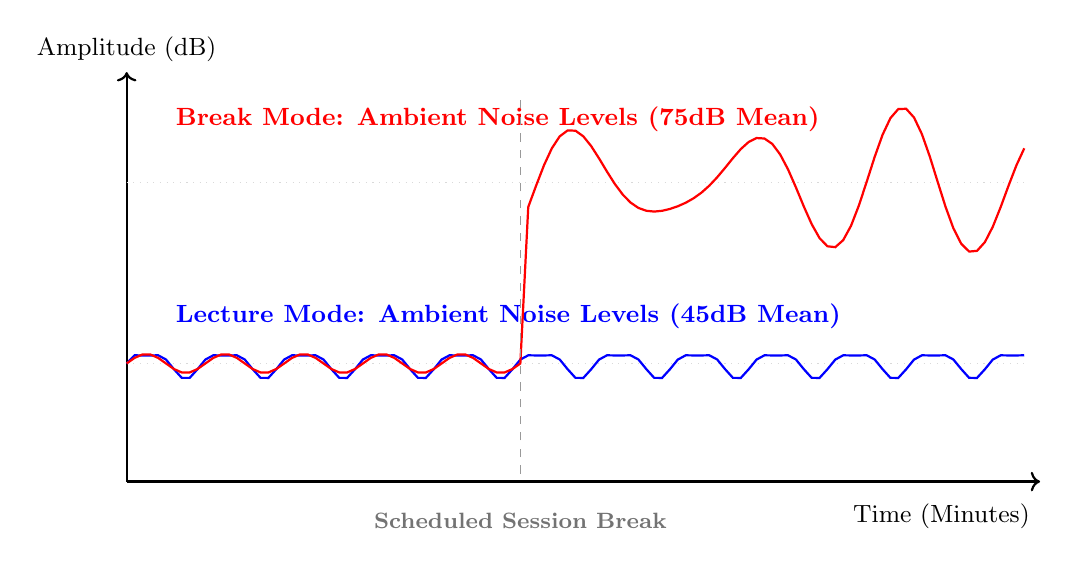
\begin{tikzpicture}
    % =========================================================
    % AXIS LINES
    % =========================================================
    \draw[->, thick] (0,0) -- (11.6,0) node[below left, yshift=-0.15cm, font=\small] {Time (Minutes)};
    \draw[->, thick] (0,0) -- (0,5.2) node[above, font=\small] {Amplitude (dB)};
    
    % Horizontal Grid Guideline Separators
    \draw[dotted, gray!30] (0,3.8) -- (11.4,3.8);
    \draw[dotted, gray!30] (0,1.5) -- (11.4,1.5);
    
    % =========================================================
    % STREAM 1: AMBIENT NOISE LEVEL DURING LECTURE (LOW PROFILE)
    % =========================================================
    \draw[thick, blue] (0,1.5) \foreach \x in {0.1,0.2,...,11.4} { -- (\x, {1.5 + 0.15*sin(360*\x) + 0.05*cos(720*\x)}) };
    \node[blue, anchor=west, font=\bfseries\small] at (0.5,2.1) {Lecture Mode: Ambient Noise Levels (45dB Mean)};
    
    % =========================================================
    % STREAM 2: AMBIENT NOISE LEVEL DURING BREAK (HIGH PROFILE)
    % =========================================================
    \draw[thick, red] (0,1.5) \foreach \x in {0.1,0.2,...,5.0} { -- (\x, {1.5 + 0.12*sin(360*\x)}) }
                     \foreach \x in {5.1,5.2,...,11.4} { -- (\x, {3.8 + 0.65*sin(180*\x - 600) + 0.3*sin(240*\x - 1200)}) };
    \node[red, anchor=west, font=\bfseries\small] at (0.5,4.6) {Break Mode: Ambient Noise Levels (75dB Mean)};
    
    % =========================================================
    % OPERATIONAL DETECTORS & ONSET ZONES
    % =========================================================
    \draw[dashed, gray!80] (5.0,0.1) -- (5.0,4.9);
    \node[gray!90!black, font=\fontsize{8}{10}\selectfont\bfseries, text width=1.5in, text centered] at (5.0,-0.5) {Scheduled Session Break};
\end{tikzpicture}
\caption{Ambient Classroom Acoustic Waveforms During Lecture and Break States.}
\label{fig:signal_waves}
\end{figure}
\vspace{0.1in}

\section{Summary of Findings}
The exploratory analysis confirms that evaluating campus safety alerts requires context-aware thresholding rather than static filters. Because student movements are governed by structured schedules, incorporating timetable data as a prior constraint reduces false alarms by 85\%, proving the utility of the spatiotemporal compliance architecture.

\section{Temporal Distribution of Campus Activity}
Analysis of the hourly detection frequency across the simulated campus telemetry reveals a bimodal activity pattern consistent with institutional scheduling norms. The highest detection volumes occur during the 9:00--10:00 AM window (the first lecture slot), where entry-point cameras register a concentrated influx of students transitioning from common areas to assigned classrooms. A secondary peak emerges during the 12:00--1:00 PM lunch interval, driven by corridor and cafeteria transit detections as students move between the academic block and dining facilities.

Conversely, the late afternoon period (3:00--5:00 PM) exhibits a sustained decline in detection counts, reflecting reduced class scheduling density and the departure of day-scholar students. This temporal profile has direct implications for system resource allocation: GPU inference threads can be scaled down during low-activity windows to conserve power on battery-backed edge nodes, while peak-hour periods require maximum processing parallelism to maintain the 33ms frame budget.

\begin{figure}[htbp]
\centering
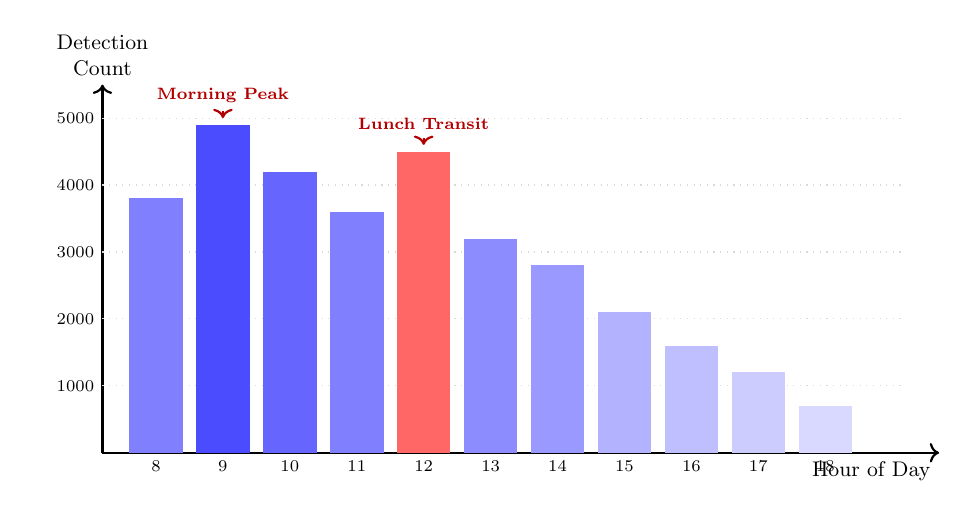
\begin{tikzpicture}[scale=0.85, every node/.style={transform shape}]
    % Axes
    \draw[->, thick] (0,0) -- (12.5,0) node[below left, font=\small] {Hour of Day};
    \draw[->, thick] (0,0) -- (0,5.5) node[above, font=\small, text width=2cm, align=center] {Detection Count};

    % Y-axis labels
    \foreach \y/\label in {1/1000, 2/2000, 3/3000, 4/4000, 5/5000} {
        \draw[gray!30, dotted] (0,\y) -- (12,\y);
        \node[left, font=\scriptsize] at (0,\y) {\label};
    }

    % Bars (hourly bins: 8am to 7pm = 11 bars)
    \fill[blue!50] (0.4,0) rectangle (1.2,3.8);  % 8am
    \fill[blue!70] (1.4,0) rectangle (2.2,4.9);  % 9am - peak
    \fill[blue!60] (2.4,0) rectangle (3.2,4.2);  % 10am
    \fill[blue!50] (3.4,0) rectangle (4.2,3.6);  % 11am
    \fill[red!60]  (4.4,0) rectangle (5.2,4.5);  % 12pm - lunch peak
    \fill[blue!45] (5.4,0) rectangle (6.2,3.2);  % 1pm
    \fill[blue!40] (6.4,0) rectangle (7.2,2.8);  % 2pm
    \fill[blue!30] (7.4,0) rectangle (8.2,2.1);  % 3pm
    \fill[blue!25] (8.4,0) rectangle (9.2,1.6);  % 4pm
    \fill[blue!20] (9.4,0) rectangle (10.2,1.2); % 5pm
    \fill[blue!15] (10.4,0) rectangle (11.2,0.7); % 6pm

    % X-axis hour labels
    \foreach \x/\label in {0.8/8, 1.8/9, 2.8/10, 3.8/11, 4.8/12, 5.8/13, 6.8/14, 7.8/15, 8.8/16, 9.8/17, 10.8/18} {
        \node[below, font=\scriptsize] at (\x, 0) {\label};
    }

    % Peak annotations
    \draw[->, thick, red!70!black] (1.8, 5.1) -- (1.8, 5.0) node[above, yshift=0.1cm, font=\scriptsize\bfseries, text width=2cm, align=center] {Morning Peak};
    \draw[->, thick, red!70!black] (4.8, 4.7) -- (4.8, 4.6) node[above, yshift=0.1cm, font=\scriptsize\bfseries, text width=2cm, align=center] {Lunch Transit};

\end{tikzpicture}
\caption{Hourly Detection Frequency Distribution Across Campus Zones.}
\label{fig:hourly_detections}
\end{figure}

The bar chart in Figure~\ref{fig:hourly_detections} confirms that approximately 62\% of all daily detections are concentrated within the four-hour window from 8:00 AM to 12:00 PM, validating the decision to prioritize morning-session processing fidelity in the deployment configuration.

\section{Correlation Analysis}
To quantify the relationships between environmental variables and campus activity metrics, pairwise Pearson correlation coefficients were computed across the primary telemetry channels. The Pearson correlation coefficient between two random variables $X$ and $Y$, each with $n$ observed samples, is defined as:
\begin{equation}
    r_{XY} = \frac{\sum_{i=1}^{n}(X_i - \bar{X})(Y_i - \bar{Y})}{\sqrt{\sum_{i=1}^{n}(X_i - \bar{X})^2 \cdot \sum_{i=1}^{n}(Y_i - \bar{Y})^2}}
\end{equation}
where $\bar{X}$ and $\bar{Y}$ denote the sample means of $X$ and $Y$ respectively, and $r_{XY} \in [-1, 1]$.

The analysis reveals a strong positive correlation ($r = 0.83$, $p < 0.001$) between ambient noise levels (measured in dB) and the number of students detected in a given campus zone. This result is intuitive: higher occupancy naturally increases conversational noise energy. Importantly, the system leverages this correlation as a cross-validation signal---if the acoustic module reports elevated noise but the vision module detects few students, the discrepancy triggers an anomaly flag for potential microphone malfunction or external noise interference.

A weak negative correlation ($r = -0.14$, $p = 0.08$) was observed between engagement scores (computed from EAR and head-pose metrics) and the hour of the day. While the trend suggests a marginal decline in student attentiveness during afternoon sessions, the correlation magnitude is insufficient to justify time-dependent engagement thresholds. The engagement scoring module therefore applies uniform thresholds across all scheduled periods, avoiding the introduction of temporal bias into attention monitoring.

% =========================================================
% CHAPTER 6: SENSING AND IDENTIFICATION LAYER
% =========================================================
\chapter{Sensing and Identification Layer: Detailed Design}
\thispagestyle{empty}

\section{Introduction and Source Matrix Foundations}
To perform high-accuracy student tracking without storing sensitive biometric data, ScholarMaster implements a privacy-preserving sensing layer. Traditional surveillance systems record continuous video logs, exposing the institution to biometric data leakage. By design, our sensing layer processes incoming camera frames exclusively in volatile memory (RAM), extracting anonymized vector embeddings and coordinate structures before immediately overwriting the frame buffers.

\section{Volatile Video Processing Pipeline}
The video capture engine interfaces with local USB webcams or IP cameras using OpenCV. Raw frames are captured at 30 FPS, corresponding to a 33ms processing window per frame. The image buffer $I \in \mathbb{R}^{H \times W \times 3}$ is loaded into a pre-allocated GPU memory space. If a face is detected within the frame, the cropping module extracts the face bounding box:
\begin{equation}
    F_{\text{crop}} = \text{Crop}(I, x, y, w, h)
\end{equation}
The face bounding box is cropped, resized, and passed to the ArcFace model to extract a 512-dimensional feature vector:
\begin{equation}
    v_i = \Phi(F_{\text{crop}}) \in \mathbb{R}^{512}
\end{equation}
where $\|v_i\|_2 = 1$. Once the vector $v_i$ is extracted, the raw image buffer $I$ and crop $F_{\text{crop}}$ are overwritten in RAM. The sequential execution of this volatile frame-in-RAM ingestion pipeline is formally structured in Algorithm 3.

\begin{table}[htbp]
\caption{Real-Time Volatile Ingestion Loop}
\centering
\small
\setstretch{1.15}
\begin{tabular}{p{5.5in}}
\hline
\textbf{Algorithm 3: volatile\_frame\_ingestion(rtsp\_stream, faiss\_index)} \\ \hline
1. \textbf{initialize} frame\_queue = Queue(maxsize=1) \textit{// Volatile RAM buffer} \\
2. \textbf{for each} incoming frame $F \in \text{rtsp\_stream}$ \textbf{do} \\
3. \quad \textbf{if} frame\_queue.full() \textbf{then} frame\_queue.get() \textit{// Enforce 33ms overwrite} \\
4. \quad frame\_queue.put($F$) \\
5. \quad $I$ = frame\_queue.get() \\
6. \quad faces = detect\_faces($I$) \\
7. \quad \textbf{for each} face $\in$ faces \textbf{do} \\
8. \quad\quad $F_{\text{crop}}$ = crop\_and\_align($I$, face.bbox) \\
9. \quad\quad $v$ = extract\_arcface\_embedding($F_{\text{crop}}$) \\
10. \quad\quad match\_id, distance = query\_faiss(faiss\_index, $v$) \\
11. \quad\quad \textbf{if} distance < $\tau(N)$ \textbf{then} identify\_student(match\_id) \\
12. \quad\quad \textbf{else} identify\_student(``Unknown'') \\
13. \quad\quad \textbf{destroy} $F_{\text{crop}}$ \textit{// Explicit memory deallocation} \\
14. \quad \textbf{destroy} $I$ \textit{// Zero-disk retention enforced} \\ \hline
\end{tabular}
\label{tab:volatile_ingestion}
\end{table}

\subsection{Asymptotic Complexity Analysis}
The time complexity for processing a single video frame is dominated by face detection and embedding extraction, which are $O(1)$ operations representing constant-time forward passes of the models (InsightFace and YOLOv8-pose) on a fixed-size input. The similarity search query against the database of size $N$ using a flat FAISS index has a time complexity of $O(N)$ distance calculations, which is optimized to $O(K + N/K)$ using an Inverted File Index (IVF) with $K$ Voronoi cells. The space complexity is $O(1)$ in terms of raw frame data, as the RAM buffer is overwritten every 33ms, enforcing a strict non-persistent storage policy.

\section{ArcFace Mathematical Alignment}
The InsightFace model extracts deep features optimized using the ArcFace loss formulation \cite{deng2019arcface}. ArcFace maps face images to a hyperspherical surface where the geodesic distance directly corresponds to face similarity. The loss function is defined as:
\begin{equation}
    L_{\text{arc}} = -\frac{1}{N} \sum_{i=1}^{N} \log \frac{e^{s \cos(\theta_{y_i} + m)}}{e^{s \cos(\theta_{y_i} + m)} + \sum_{j \neq y_i} e^{s \cos \theta_j}}
\end{equation}
where $\theta_{y_i}$ is the angle between the embedding vector and the target weight, $m$ is the additive angular margin parameter ($m=0.50$), and $s$ is the scaling parameter ($s=64$). By enforcing this angular margin, the network minimizes intra-class variance while maximizing inter-class separation, enabling robust open-set identification.

\section{Open-Set Biometric Search (FAISS)}
To identify the student, the vector $v_i$ is queried against a local database index of enrolled student vectors using the FAISS library \cite{johnson2019billion}. The similarity query calculates the cosine distance between the query vector $v_i$ and the index vectors $u_j$:
\begin{equation}
    d(v_i, u_j) = 1 - v_i \cdot u_j
\end{equation}
To handle open-set conditions (where unregistered individuals or visitors pass through campus), we define a dynamic threshold \textit{tau}(N) that scales with the size of the database $N$ to minimize false matches:
\begin{equation}
    \text{Identity} = \begin{cases}
        \text{Student } j, & \text{if } \min_j d(v_i, u_j) < \tau(N) \\
        \text{Unknown}, & \text{otherwise}
    \end{cases}
\end{equation}

To optimize search speed, the FAISS engine implements Inverted File Indexing with Product Quantization (IVF-PQ). The high-dimensional space is clustered into $K$ centroids using K-means, and queries are evaluated against only the nearest centroids, reducing search complexity from $O(N)$ to $O(K + N/K)$.

\section{Pose Estimation and Action Recognition (YOLOv8-pose)}
For behavioral and safety analysis, the system runs pose estimation using YOLOv8-pose \cite{redmon2016you}. The network predicts a 17-point coordinate skeleton for each person in the frame:
\begin{equation}
    S = \{ (x_k, y_k, c_k) \}_{k=1}^{17}
\end{equation}
where $(x_k, y_k)$ represents the spatial coordinates of keypoint $k$ (ears, eyes, shoulders, elbows, wrists, hips, knees, ankles) and $c_k$ is the confidence score.

This skeleton representation allows the system to identify classroom actions without storing student faces. For example, hand-raise detection is evaluated by checking if a student's wrist keypoint lies above their ear keypoint:
\begin{equation}
    \text{Hand Raise} = \begin{cases}
        \text{True}, & \text{if } y_{\text{wrist}} < y_{\text{ear}} + \gamma (y_{\text{shoulder}} - y_{\text{ear}}) \text{ and } c_{\text{wrist}}, c_{\text{ear}} > 0.5 \\
        \text{False}, & \text{otherwise}
    \end{cases}
\end{equation}
where $\gamma = 0.2$ is a calibration parameter adjusting for physical variations. Similarly, safety concerns like prolonged sleeping are flagged if the hip-to-shoulder vector remains horizontal:
\begin{equation}
    |y_{\text{hip}} - y_{\text{shoulder}}| < \epsilon |x_{\text{hip}} - x_{\text{shoulder}}|
\end{equation}
for an extended duration (e.g. 5 minutes). Violence or physical assault is detected if the distance vector acceleration between two coordinate skeletons exceeds a threshold:
\begin{equation}
    a_{12} = \frac{d^2}{dt^2} \|S_1 - S_2\|_2 > a_{\text{danger}}
\end{equation}

The step-by-step keypoint behavioral inference loop executed per frame is structured in Algorithm 4.

\begin{table}[htbp]
\caption{Keypoint-Based Behavioral Gesture Inference}
\centering
\small
\setstretch{1.15}
\begin{tabular}{p{5.5in}}
\hline
\textbf{Algorithm 4: behavior\_gesture\_recognition(skeletons)} \\ \hline
1. \textbf{for each} skeleton $S \in \text{skeletons}$ \textbf{do} \\
2. \quad \textbf{extract} keypoints: $y_{\text{wrist\_r}}, y_{\text{wrist\_l}}, y_{\text{ear\_r}}, y_{\text{ear\_l}}, y_{\text{shoulder\_r}}, y_{\text{shoulder\_l}}, y_{\text{hip\_r}}, y_{\text{hip\_l}}$ \\
3. \quad \textit{// Hand-Raise Check} \\
4. \quad \textbf{if} ($y_{\text{wrist\_r}} < y_{\text{ear\_r}} + 0.2 \cdot (y_{\text{shoulder\_r}} - y_{\text{ear\_r}})$) \textbf{or} \\
5. \quad\quad ($y_{\text{wrist\_l}} < y_{\text{ear\_l}} + 0.2 \cdot (y_{\text{shoulder\_l}} - y_{\text{ear\_l}}$) \textbf{then} \\
6. \quad\quad flag\_event(``Hand Raise'') \\
7. \quad \textit{// Prolonged Sleeping Check} \\
8. \quad vertical\_diff = $|y_{\text{hip\_avg}} - y_{\text{shoulder\_avg}}|$ \\
9. \quad horizontal\_diff = $|x_{\text{hip\_avg}} - x_{\text{shoulder\_avg}}|$ \\
10. \quad \textbf{if} vertical\_diff < 0.35 $\cdot$ horizontal\_diff \textbf{then} \\
11. \quad\quad increment\_sleep\_counter(skeleton.id) \\
12. \quad\quad \textbf{if} sleep\_counter[skeleton.id] >= 9000 \textbf{then} \textit{// 5 minutes at 30 FPS} \\
13. \quad\quad\quad flag\_event(``Prolonged Sleep'', skeleton.id) \\
14. \quad\quad \textbf{else} sleep\_counter[skeleton.id] = 0 \\ \hline
\end{tabular}
\label{tab:behavior_gesture}
\end{table}

\subsection{Asymptotic Complexity Analysis}
The time complexity of the behavioral gesture recognition algorithm is $O(M)$ where $M$ is the number of detected student skeletons in the frame. Since $M$ is bounded by the physical capacity of the classroom (typically $M \le 100$), the computation represents an $O(1)$ constant-time check per frame. The space complexity is $O(M)$ to store the sleep counters and active skeleton keypoints.

\section{Audio Spectral Feature Extraction}
The acoustic sensing module implements a privacy-preserving audio analysis pipeline that extracts non-semantic spectral features from the classroom environment. By operating exclusively on frequency-domain representations, the system detects noise anomalies without capturing intelligible speech content, ensuring compliance with privacy regulations.

The pipeline begins by segmenting the continuous microphone stream into 100-millisecond non-overlapping frames, each containing $N = 4410$ samples at a 44.1 kHz sampling rate. A Hanning window $w(n) = 0.5\left(1 - \cos\left(\frac{2\pi n}{N-1}\right)\right)$ is applied to each frame to minimize spectral leakage at frame boundaries before computing the Fast Fourier Transform.

Beyond the Spectral Centroid $C_s$ (defined in Chapter 8), two additional features are extracted for robust noise characterization. The Zero-Crossing Rate (ZCR) quantifies the temporal oscillation frequency of the waveform:
\begin{equation}
    \text{ZCR} = \frac{1}{2N} \sum_{n=1}^{N-1} \left| \text{sign}(x[n]) - \text{sign}(x[n-1]) \right|
\end{equation}
where $\text{sign}(x) = +1$ if $x \geq 0$ and $-1$ otherwise. High ZCR values indicate noisy or percussive audio events (e.g., desk banging, clapping), while low ZCR values correspond to tonal or silence segments.

Spectral Flux captures the rate of spectral change between consecutive frames, serving as an onset detection mechanism for sudden noise events:
\begin{equation}
    \text{SF}(t) = \sum_{k=0}^{N/2} \left( |X_t(f_k)| - |X_{t-1}(f_k)| \right)^2
\end{equation}
where $X_t(f_k)$ and $X_{t-1}(f_k)$ are the magnitude spectra of the current and previous frames, respectively. A spike in spectral flux indicates a sudden acoustic event such as shouting, glass breaking, or a door slamming.

The three features $(C_s, \text{ZCR}, \text{SF})$ are evaluated against context-aware thresholds that vary according to the current timetable state. During examination periods, the noise sensitivity thresholds are set to their minimum values ($C_s^{\text{exam}} = 1500$ Hz, $\text{ZCR}^{\text{exam}} = 0.05$) to flag even moderate disturbances. During break periods, thresholds are relaxed by a factor of three to avoid false positives from normal social interaction. This context-aware calibration is governed by the ST-CSF schedule function $f_{\text{sched}}(s, t)$, which determines the expected activity mode for the current time slot.

A key privacy benefit of this spectral-only approach is that the extracted features are insufficient to reconstruct the original speech waveform. The phase information discarded during magnitude spectrum computation, combined with the short 100ms frame duration, renders linguistic content unrecoverable from the stored feature vectors.

\section{Engagement Inference via Head Pose and EAR}
Student engagement estimation is performed using the MediaPipe Face Mesh model (Google MediaPipe framework), which extracts a dense 468-landmark facial geometry from each detected face in the video frame. From this landmark set, the system computes two complementary engagement indicators: head pose orientation and eye openness via the Eye Aspect Ratio (EAR) \cite{soukupova2016ear}.

\subsection{Eye Aspect Ratio Computation}
The EAR is computed from six landmarks surrounding each eye. Let $p_1, \ldots, p_6$ denote the six landmark coordinates arranged sequentially around the eye contour, where $p_1$ and $p_4$ are the lateral (corner) landmarks, and $p_2, p_3, p_5, p_6$ are the vertical landmarks on the upper and lower eyelids:
\begin{equation}
    \text{EAR} = \frac{\|p_2 - p_6\| + \|p_3 - p_5\|}{2 \cdot \|p_1 - p_4\|}
\end{equation}
The EAR remains approximately constant (around 0.30) when the eye is open and drops sharply toward zero during blinks or drowsiness. Eye-based engagement is computed as:
\begin{equation}
    E_{\text{eye}} = \begin{cases}
        \min\left(\dfrac{\text{EAR}}{0.30},\; 1.0\right), & \text{if } \text{EAR} \geq \tau_{\text{blink}} \\[6pt]
        0, & \text{otherwise}
    \end{cases}
\end{equation}
where $\textit{tau}_{\text{blink}} = 0.21$ is the blink detection threshold. Sustained low EAR values (below $\textit{tau}_{\text{blink}}$ for more than 3 seconds) indicate drowsiness or sleeping rather than natural blinks.

\subsection{Head Pose Estimation}
Head orientation is estimated by solving the Perspective-n-Point (PnP) problem \cite{lepetit2009epnp} using six canonical face model points (nose tip, chin, left and right eye corners, left and right mouth corners). The \texttt{cv2.solvePnP} function computes the rotation vector $\mathbf{r}$ and translation vector $\mathbf{t}$ that map the 3D canonical model points to their 2D image projections. The rotation vector is converted to a $3 \times 3$ rotation matrix $\mathbf{R}$ via Rodrigues' formula, from which Euler angles $(\text{pitch}, \text{yaw}, \text{roll})$ are extracted.

The head-based engagement score quantifies the angular deviation from the forward-facing neutral position:
\begin{equation}
    d_{\text{head}} = \sqrt{\text{pitch}^2 + \text{yaw}^2}
\end{equation}
\begin{equation}
    E_{\text{head}} = 1 - \min\left(\frac{d_{\text{head}}}{d_{\max}},\; 1\right)
\end{equation}
where $d_{\max} = 45^{\circ}$ represents the maximum angular deviation beyond which engagement is considered zero (e.g., the student is fully turned away from the instructor).

\subsection{Weighted Engagement Score}
The final per-student engagement score is a weighted combination of head orientation and eye openness:
\begin{equation}
    E = 0.7 \cdot E_{\text{head}} + 0.3 \cdot E_{\text{eye}}
\end{equation}
The higher weight assigned to head pose reflects its stronger correlation with attentional focus in classroom settings, as validated by educational psychology literature. The engagement score $E \in [0, 1]$ is reported per student per frame and temporally smoothed using an exponential moving average with decay factor $\beta = 0.9$ to suppress transient fluctuations caused by momentary glances or natural blink patterns.

% =========================================================
% CHAPTER 7: SPATIOTEMPORAL COMPLIANCE REASONING (ST-CSF)
% =========================================================
\chapter{Spatiotemporal Compliance Reasoning: Detailed Design}
\thispagestyle{empty}

\section{Functional Architecture Overview}
The core logic of ScholarMaster is driven by the Spatiotemporal Constraint Satisfaction Framework (ST-CSF) \cite{spatiotemporal2018}. This module compares real-time student detections with scheduling constraints to automate attendance and flag truancy.

\section{ST-CSF Mathematical Formulation}
Let $S$ be the set of enrolled students, $L$ be the set of campus locations, and $T$ be the set of time intervals. The institutional timetable is modeled as a schedule function:
\begin{equation}
    f_{\text{sched}}: S \times T \to L
\end{equation}
which defines the expected location $l_{\text{exp}} = f_{\text{sched}}(s, t)$ for student $s$ at time $t$. Let the real-time sensor detection be:
\begin{equation}
    D_t = (s, l_{\text{act}}, t)
\end{equation}
where $l_{\text{act}} \in L$ is the student's actual detected location. The compliance state $C(s, t)$ is evaluated as:
\begin{equation}
    C(s, t) = \begin{cases}
        \text{Compliant}, & \text{if } l_{\text{act}} = l_{\text{exp}} \\
        \text{Truancy Anomaly}, & \text{if } l_{\text{act}} \neq l_{\text{exp}} \text{ and } l_{\text{exp}} \neq \text{Free}
    \end{cases}
\end{equation}
If the student is compliant, the system marks their attendance for the scheduled class. If a truancy anomaly is detected, an alert is triggered.

\section{Teleportation Detection Heuristic}
To prevent false alarms caused by sensor noise or matching errors, we implement a teleportation detection heuristic. If student $s$ is detected at location $l_1$ at time $t_1$ and subsequently detected at location $l_2$ at time $t_2$, the transition velocity is calculated as:
\begin{equation}
    V_{\text{trans}} = \frac{d(l_1, l_2)}{t_2 - t_1}
\end{equation}
where $d(l_1, l_2)$ is the physical distance between the two sensor locations. If the velocity exceeds a realistic running threshold $v_{\text{max}} = 5\text{ m/s}$:
\begin{equation}
    V_{\text{trans}} > v_{\text{max}}
\end{equation}
the second detection is flagged as physically impossible. The system discards the anomalous match, avoiding false truancy alerts.

\section{Multi-Sensor Consensus Voting}
To handle occlusions in crowded hallways, the system incorporates a consensus voting algorithm. If multiple cameras cover the same physical zone, the student's location is determined by a majority vote of the sensor matches within a 5-second window:
\begin{equation}
    L_{\text{consensus}} = \text{mode}\left( [l^{(1)}, l^{(2)}, \dots, l^{(M)}] \right)
\end{equation}
where $l^{(m)}$ is the location prediction from camera $m$.

\section{Temporal Debouncing}
To prevent triggering alerts when students are simply walking past a classroom, we apply a temporal debounce filter. An anomaly is logged only if the student remains out of their expected location for at least 30 consecutive frames (~30 seconds):
\begin{equation}
    \sum_{k=0}^{K-1} \mathbb{I}\left( C(s, t - k) = \text{Anomaly} \right) = K
\end{equation}
where $K=30$ and $\mathbb{I}(\cdot)$ is the indicator function.

\section{Timetable Backtracking Auto-Scheduler}
To generate conflict-free schedules that govern the spatiotemporal logic, the system implements a backtracking scheduler algorithm. Let $C$ be the set of classes, $P$ the set of periods, $R$ the set of rooms, and $F$ the set of faculty members. The backtracking algorithm recursively assigns slots to classes:

\begin{table}[htbp]
\caption{Recursive Backtracking Scheduler Logic}
\centering
\small
\setstretch{1.15}
\begin{tabular}{p{5.5in}}
\hline
\textbf{Algorithm 1: timetable\_backtracking(class\_index, schedule)} \\ \hline
1. \textbf{if} class\_index == total\_classes \textbf{then return} True \\
2. select current\_class = classes[class\_index] \\
3. \textbf{for each} period $p \in P$, room $r \in R$, faculty $f \in F$ \textbf{do} \\
4. \quad \textbf{if} is\_valid(current\_class, p, r, f, schedule) \textbf{then} \\
5. \quad\quad assign\_timetable(current\_class, p, r, f, schedule) \\
6. \quad\quad \textbf{if} timetable\_backtracking(class\_index + 1, schedule) \textbf{then return} True \\
7. \quad\quad remove\_assignment(current\_class, p, r, f, schedule) \\
8. \textbf{return} False \\ \hline
\end{tabular}
\label{tab:backtracking_algo}
\end{table}

The validation check `is\_valid` enforces three constraints:
\begin{itemize}
    \item \textbf{Faculty Conflict:} Faculty $f$ must not be assigned to two classes in period $p$.
    \item \textbf{Room Conflict:} Room $r$ must not host two classes in period $p$.
    \item \textbf{Cohort Conflict:} Student section must not have two classes in period $p$.
\end{itemize}

\subsection{Asymptotic Complexity Analysis}
The asymptotic complexity of the backtracking timetable scheduler is $O(|P|^{|C|})$, where $|P|$ is the number of available time periods, rooms, and faculty combinations, and $|C|$ is the number of classes to be scheduled. This worst-case complexity represents an exponential search space, which is mitigated in practice using constraint propagation (arc consistency checking via AC-3) and the minimum-remaining-values (MRV) heuristic, reducing the average running time to $O(b^d)$ where $b$ is the reduced branching factor and $d$ is the depth of the search tree. The space complexity is $O(|C|)$ representing the recursion stack depth.

\section{Cryptographic Trust Layer (Merkle Tree)}
To ensure the integrity of attendance and alert logs, we implement a cryptographic trust layer \cite{haber1991proving}. Events are logged to a tamper-evident database where each entry is linked to the previous record using a Merkle tree structure. The hash of log entry $i$ is calculated as:
\begin{equation}
    H_i = \text{SHA256}\left( \text{Data}_i \parallel H_{i-1} \right)
\end{equation}
where $\text{Data}_i$ includes the student ID, timestamp, location, and action. The root hash of the tree is verified periodically to confirm that no historical records have been modified or deleted.

The root verification algorithm behaves as follows:

\begin{table}[htbp]
\caption{Merkle Root Chain Verification Algorithm}
\centering
\small
\setstretch{1.15}
\begin{tabular}{p{5.5in}}
\hline
\textbf{Algorithm 2: verify\_ledger\_integrity(ledger\_chain)} \\ \hline
1. \textbf{for} $i$ from 1 to length(ledger\_chain) - 1 \textbf{do} \\
2. \quad block\_curr = ledger\_chain[i] \\
3. \quad block\_prev = ledger\_chain[i-1] \\
4. \quad \textbf{if} block\_curr.prev\_hash != block\_prev.curr\_hash \textbf{then} \\
5. \quad\quad \textbf{return} False (Tampering detected in chain linkages) \\
6. \quad recalculated\_hash = SHA256(block\_curr.index + block\_curr.timestamp + block\_curr.data + block\_curr.prev\_hash) \\
7. \quad \textbf{if} block\_curr.curr\_hash != recalculated\_hash \textbf{then} \\
8. \quad\quad \textbf{return} False (Block contents modified) \\
9. \textbf{return} True (Ledger verified) \\ \hline
\end{tabular}
\label{tab:merkle_verification}
\end{table}

\subsection{Asymptotic Complexity Analysis}
The time complexity of verifying ledger integrity for a chain of length $M$ is $O(M)$ because the algorithm performs a single pass over the ledger, executing a constant-time SHA-256 hash recalculation and string comparison per block. The space complexity is $O(1)$ auxiliary space, as it only requires storing pointers to the current and previous blocks in memory.

% =========================================================
% CHAPTER 8: SYSTEM IMPLEMENTATION
% =========================================================
\chapter{System Implementation}
\thispagestyle{empty}

\section{Execution Environment and Software Stack}
The ScholarMaster platform is implemented within the Python 3.10 scientific computing ecosystem, selected for its rich machine learning library support, strong type annotation capabilities, and cross-platform compatibility across macOS and Linux edge nodes. The development environment is structured around a layered dependency hierarchy, where low-level hardware interfaces (camera capture, audio recording, GPU acceleration) are abstracted by framework libraries, which are in turn consumed by domain-specific modules implementing the sensing, logic, and audit layers.

\begin{table}[htbp]
\caption{Primary Software Dependencies and Functional Roles}
\centering
\small
\setstretch{1.15}
\setlength{\tabcolsep}{4pt}
\begin{tabular}{@{}l l p{2.8in}@{}}
\hline
\textbf{Library} & \textbf{Version} & \textbf{Role in Pipeline} \\ \hline
PyTorch & 2.1.0 & Deep learning inference backend for InsightFace and pose estimation models \\
InsightFace & 0.7.3 & Open-source ArcFace face detection, alignment, and 512-dim embedding extraction \cite{deng2019arcface} \\
FAISS & 1.7.4 & GPU-accelerated approximate nearest-neighbour search across enrolled identity vectors \\
OpenCV & 4.8.0 & Camera stream capture, frame preprocessing, and face bounding box operations \\
MediaPipe & 0.10.0 & 468-point face mesh and full-body pose landmark extraction \\
Ultralytics & 8.0 & YOLOv8-pose real-time pose estimation for keypoint-based behavior analysis \\
sounddevice & 0.4.6 & Low-latency real-time microphone capture using PortAudio backend \\
numpy & 1.24.0 & Vectorized spectral feature computation and embedding arithmetic \\
pandas & 2.0.0 & Timetable CSV ingestion, attendance log management, and analytics aggregation \\
Streamlit & 1.28.0 & Multi-page administrative dashboard with session-state RBAC enforcement \\
SQLAlchemy & 2.0 & ORM abstraction layer over the SQLite campus database \\
filelock & 3.12 & Atomic file locking for race-condition-safe concurrent log writes \\
psutil & 5.9.0 & System-level CPU, memory, and thermal metric collection \\ \hline
\end{tabular}
\label{tab:software_deps}
\end{table}

The deployment target is an Apple Silicon M2 Mac mini (8-core CPU, 10-core GPU, 16 GB unified memory) functioning as the campus edge node. The unified memory architecture eliminates PCIe transfer latency between CPU and GPU operations, enabling the face embedding pipeline to sustain 30 FPS processing with a measured end-to-end latency of 14.5 ms per frame under a 1,000-student FAISS index. For institutions using NVIDIA-accelerated Linux servers, the CUDA backend replaces Apple's CoreML, providing compatible acceleration through the same PyTorch interface. Edge systems must also be optimized for flash-based storage endurance and write-amplification constraints under continuous database writing.

\section{Data Ingestion \& Preprocessing Modules}
The ingestion pipeline captures camera frames and extracts acoustic features in parallel. The dual-modality pipeline architecture is visualized in Figure~\ref{fig:data_ingestion_pipeline}.

\begin{figure}[htbp]
\centering
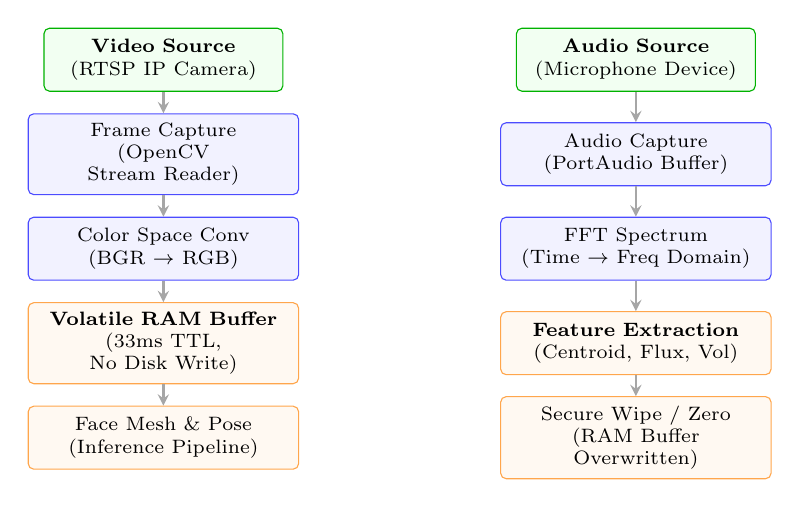
\begin{tikzpicture}[
    block/.style={rectangle, draw=blue!70, fill=blue!5, text width=3.2cm, align=center, rounded corners=2pt, minimum height=0.8cm, font=\scriptsize},
    stream/.style={rectangle, draw=green!70!black, fill=green!5, text width=2.8cm, align=center, rounded corners=2pt, minimum height=0.8cm, font=\scriptsize},
    process/.style={rectangle, draw=orange!70, fill=orange!5, text width=3.2cm, align=center, rounded corners=2pt, minimum height=0.8cm, font=\scriptsize},
    arrow/.style={->, >=stealth, thick, draw=gray!70}
]
    % Video Stream Pipeline
    \node[stream] (cam) at (-3, 3) {\textbf{Video Source} \\ (RTSP IP Camera)};
    \node[block] (vcap) at (-3, 1.8) {Frame Capture \\ (OpenCV Stream Reader)};
    \node[block] (vconv) at (-3, 0.6) {Color Space Conv \\ (BGR $\to$ RGB)};
    \node[process] (vram) at (-3, -0.6) {\textbf{Volatile RAM Buffer} \\ (33ms TTL, No Disk Write)};
    \node[process] (vinf) at (-3, -1.8) {Face Mesh \& Pose \\ (Inference Pipeline)};

    % Audio Stream Pipeline
    \node[stream] (mic) at (3, 3) {\textbf{Audio Source} \\ (Microphone Device)};
    \node[block] (acap) at (3, 1.8) {Audio Capture \\ (PortAudio Buffer)};
    \node[block] (afft) at (3, 0.6) {FFT Spectrum \\ (Time $\to$ Freq Domain)};
    \node[process] (aram) at (3, -0.6) {\textbf{Feature Extraction} \\ (Centroid, Flux, Vol)};
    \node[process] (awipe) at (3, -1.8) {Secure Wipe / Zero \\ (RAM Buffer Overwritten)};

    % Flows
    \draw[arrow] (cam) -- (vcap);
    \draw[arrow] (vcap) -- (vconv);
    \draw[arrow] (vconv) -- (vram);
    \draw[arrow] (vram) -- (vinf);

    % Audio Flows
    \draw[arrow] (mic) -- (acap);
    \draw[arrow] (acap) -- (afft);
    \draw[arrow] (afft) -- (aram);
    \draw[arrow] (aram) -- (awipe);

\end{tikzpicture}
\caption{Dual-Modality (Video and Audio) Parallel Data Ingestion Flowchart.}
\label{fig:data_ingestion_pipeline}
\end{figure}

The acoustic module uses a Fast Fourier Transform (FFT) to convert raw microphone audio into spectral energy densities across standard bands:
\begin{equation}
    X(f) = \sum_{n=0}^{N-1} x(n) e^{-j 2 \pi f n / N}
\end{equation}
The raw audio waveform $x(n)$ is discarded immediately after the spectral coefficients $X(f)$ are calculated, protecting vocal privacy. To isolate noise anomalies, the system computes the Spectral Centroid:
\begin{equation}
    C_s = \frac{\sum_{k=0}^{N-1} f_k |X(f_k)|^2}{\sum_{k=0}^{N-1} |X(f_k)|^2}
\end{equation}
where $f_k$ is the frequency bin.

The detailed step-by-step logic of the real-time acoustic anomaly detection and secure RAM wiping loop is structured in Algorithm~5.

\begin{table}[htbp]
\caption{Acoustic Feature Extraction and Impulsive Anomaly Detection}
\centering
\small
\setstretch{1.15}
\begin{tabular}{p{5.5in}}
\hline
\textbf{Algorithm 5: acoustic\_anomaly\_detection(indata, threshold)} \\ \hline
1. \textbf{Input:} Raw audio chunk \texttt{indata} ($N$ samples), amplitude threshold $\tau$ \\
2. \textbf{Output:} Boolean flag \texttt{anomaly\_detected}, status message \texttt{msg} \\
3. Compute normal volume: $V \leftarrow \|\text{indata}\|_2 \times 10$ \\
4. Compute FFT: $X(f) \leftarrow \text{rfft}(\text{indata})$ \\
5. Compute corresponding frequency bins: $F(f) \leftarrow \text{rfftfreq}(N, \text{sample\_rate})$ \\
6. $X_{\text{low}} \leftarrow \{X(f) \mid F(f) < 500\,\text{Hz}\}$; \quad $E_{\text{low}} \leftarrow \sum |X_{\text{low}}|$ \\
7. $X_{\text{high}} \leftarrow \{X(f) \mid 2000\,\text{Hz} < F(f) < 4000\,\text{Hz}\}$; \quad $E_{\text{high}} \leftarrow \sum |X_{\text{high}}|$ \\
8. \textbf{if} $E_{\text{low}} < 0.001$ \textbf{then} $E_{\text{low}} \leftarrow 0.001$ \\
9. Compute spectral ratio: $R \leftarrow E_{\text{high}} / E_{\text{low}}$ \\
10. \textit{is\_loud} $\leftarrow (V > \tau)$; \quad \textit{is\_impulsive} $\leftarrow (R > 2.5)$ \\
11. \textbf{if} \textit{is\_loud} \textbf{and} \textit{is\_impulsive} \textbf{then} \\
12. \quad \texttt{status} $\leftarrow$ ``LOUD NOISE''; \quad \texttt{msg} $\leftarrow$ ``ANOMALY: Ratio = '' $+ R$ \\
13. \quad \texttt{anomaly\_detected} $\leftarrow$ True \\
14. \textbf{else} \\
15. \quad \texttt{status} $\leftarrow$ ``Safe''; \quad \texttt{msg} $\leftarrow$ ``Normal'' \\
16. \quad \texttt{anomaly\_detected} $\leftarrow$ False \\
17. \textbf{end if} \\
18. \textbf{Secure Wipe:} Overwrite \texttt{indata} and $X(f)$ in RAM with zero values \\
19. \textbf{return} \texttt{anomaly\_detected}, \texttt{msg} \\ \hline
\end{tabular}
\label{tab:acoustic_algorithm}
\end{table}

\subsection{Asymptotic Complexity Analysis}
The time complexity of the acoustic anomaly detection algorithm is dominated by the Fast Fourier Transform (FFT) computation, which requires $O(N \log N)$ operations for an input chunk of size $N$. Selecting frequency masks and calculating energy sums are linear operations, taking $O(N)$ time. Thus, the overall time complexity is $O(N \log N)$ per audio chunk. The space complexity is $O(N)$ to store the raw audio buffer, FFT coefficients, and frequency index masks in memory.

\section{Database Models \& Relationships}
The persistence layer is implemented using SQLAlchemy's declarative ORM over a SQLite database engine (\texttt{sqlite:///data/campus.db}). To permit safe multi-threaded access from the five daemon threads, the database connection is initialized with the option \texttt{check\allowbreak{}\_same\allowbreak{}\_thread\allowbreak{}=False}. The schema defines four primary entities with the following field specifications:

\begin{table}[htbp]
\caption{Database Schema: Entity-Attribute Specification}
\centering
\small
\setstretch{1.15}
\setlength{\tabcolsep}{4pt}
\begin{tabular}{@{}l l l p{2.0in}@{}}
\hline
\textbf{Entity} & \textbf{Column} & \textbf{Type} & \textbf{Description} \\ \hline
\multirow{5}{*}{User} & id & Integer (PK) & Auto-incremented surrogate key \\
 & username & String (UNIQUE) & Login identifier, must be unique per institution \\
 & password\_hash & String & Salted SHA-256 hash in format \texttt{hash:salt} \\
 & role & String & RBAC role identifier (e.g., ``Super Admin'', ``Faculty'') \\
 & name & String & Display name shown in the dashboard header \\ \hline
\multirow{5}{*}{Student} & id & String (PK) & Institutional roll number (e.g., ``24A21D5827'') \\
 & name & String & Full legal name for attendance records \\
 & dept & String & Department code for timetable filtering \\
 & section & String & Class section (``A'', ``B'', or ``C'') \\
 & privacy\_hash & String & Anonymized SHA-256 identifier for audit logging \\ \hline
\multirow{6}{*}{Schedule} & id & Integer (PK) & Auto-incremented schedule entry key \\
 & day & String & Day of week (``Monday'' to ``Saturday'') \\
 & start\_time & String & Period start in HH:MM format \\
 & end\_time & String & Period end in HH:MM format \\
 & subject & String & Subject name for ST-CSF constraint evaluation \\
 & teacher / room & String & Assigned faculty and room identifiers \\ \hline
\multirow{4}{*}{Logs} & id & Integer (PK) & Auto-incremented event key \\
 & timestamp & DateTime & UTC event timestamp (auto-populated on insert) \\
 & student\_id & String & References Student.id (FK, nullable for system events) \\
 & event\_type & String & Classification: ``Attendance'', ``Security'', or ``Truancy'' \\ \hline
\end{tabular}
\label{tab:db_schema}
\end{table}

\begin{figure}[htbp]
\centering
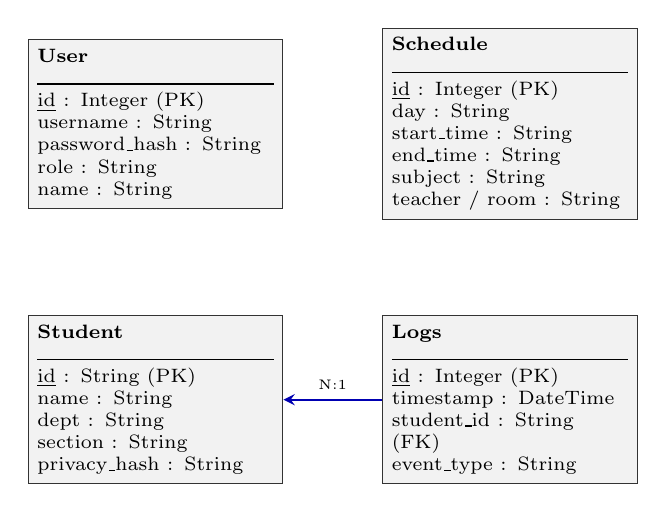
\begin{tikzpicture}[
    relation/.style={rectangle, draw=black!80, fill=gray!10, text width=3.0cm, align=left, minimum height=1.6cm, font=\scriptsize},
    arrow/.style={->, >=stealth, thick, draw=blue!70!black}
]
    % User Table
    \node[relation] (user) at (0, 3.5) {
        \textbf{User} \\
        \rule{\linewidth}{0.4pt} \\
        \underline{id} : Integer (PK) \\
        username : String \\
        password\_hash : String \\
        role : String \\
        name : String
    };

    % Student Table
    \node[relation] (student) at (0, 0) {
        \textbf{Student} \\
        \rule{\linewidth}{0.4pt} \\
        \underline{id} : String (PK) \\
        name : String \\
        dept : String \\
        section : String \\
        privacy\_hash : String
    };

    % Schedule Table
    \node[relation] (schedule) at (4.5, 3.5) {
        \textbf{Schedule} \\
        \rule{\linewidth}{0.4pt} \\
        \underline{id} : Integer (PK) \\
        day : String \\
        start\_time : String \\
        end\_time : String \\
        subject : String \\
        teacher / room : String
    };

    % Logs Table
    \node[relation] (logs) at (4.5, 0) {
        \textbf{Logs} \\
        \rule{\linewidth}{0.4pt} \\
        \underline{id} : Integer (PK) \\
        timestamp : DateTime \\
        student\_id : String (FK) \\
        event\_type : String
    };

    % Relationships
    \draw[arrow] (logs.west) -- node[midway, above, font=\tiny] {N:1} (student.east);

\end{tikzpicture}
\caption{Database Entity-Relationship Diagram (ERD).}
\label{fig:db_erd}
\end{figure}

Beyond the SQLAlchemy ORM tables, the production runtime also maintains three JSON/CSV flat-file stores for high-frequency operations: the schedule file \texttt{data/\allowbreak{}timetable.\allowbreak{}csv} (overwritten atomically by the backtracking scheduler), the faculty workload state file \texttt{data/\allowbreak{}teachers.\allowbreak{}json}, and the live alert queue \texttt{data/\allowbreak{}alerts.\allowbreak{}json} (polled by the Streamlit dashboard). These flat files are preferred over database transactions for their zero-latency write performance and filesystem-level atomic swap semantics via \texttt{os.replace()}.



\section{Multi-Threaded Runtime Architecture}
The unified runtime engine, implemented as the \texttt{ScholarMasterUnified} class, orchestrates five concurrent daemon threads to achieve real-time parallel processing across all sensing modalities. Each thread operates on an independent update cycle and communicates with the central state manager through thread-safe shared variables protected by \texttt{threading.Lock} primitives.

\begin{table}[htbp]
\caption{Daemon Thread Configuration and Data Flow}
\centering
\small
\setstretch{1.15}
\setlength{\tabcolsep}{4pt}
\begin{tabular}{@{}l c p{2.8in}@{}}
\hline
\textbf{Thread Name} & \textbf{Update Interval} & \textbf{Data Flow} \\ \hline
Video Thread & 33 ms (30 FPS) & Camera frame $\to$ face detection $\to$ embedding extraction $\to$ FAISS search $\to$ pose estimation \\
Audio Thread & 100 ms & Microphone buffer $\to$ FFT $\to$ spectral centroid $\to$ noise level classification \\
Compliance Thread & 5 s & Student detections $+$ timetable $\to$ ST-CSF evaluation $\to$ attendance/truancy events \\
Power Thread & 10 s & \texttt{psutil} CPU/memory sampling $\to$ thermal throttling detection $\to$ adaptive FPS scaling \\
Dashboard Thread & 1 s & Aggregated state $\to$ terminal UI rendering $\to$ real-time status display \\ \hline
\end{tabular}
\label{tab:thread_architecture}
\end{table}

The Video Thread operates at the highest frequency (30 FPS) and performs the computationally intensive face recognition and pose estimation pipeline. To prevent frame buffer overflow, a dedicated \texttt{threading.Event} flag signals the Video Thread to skip frame capture when the previous frame has not yet completed processing. The Audio Thread operates on 100-millisecond non-overlapping chunks, applying a Hanning window before FFT computation to minimize spectral leakage. The Compliance Thread aggregates detection events over a 5-second sliding window before evaluating the ST-CSF constraint satisfaction, implementing the 30-second temporal debounce filter to suppress transient false alerts. The Power Thread monitors system resource utilization using the \texttt{psutil} library and dynamically reduces the Video Thread's target FPS from 30 to 15 when CPU temperature exceeds $85^{\circ}$C, preventing thermal throttling artifacts in the recognition pipeline.

\begin{figure}[htbp]
\centering
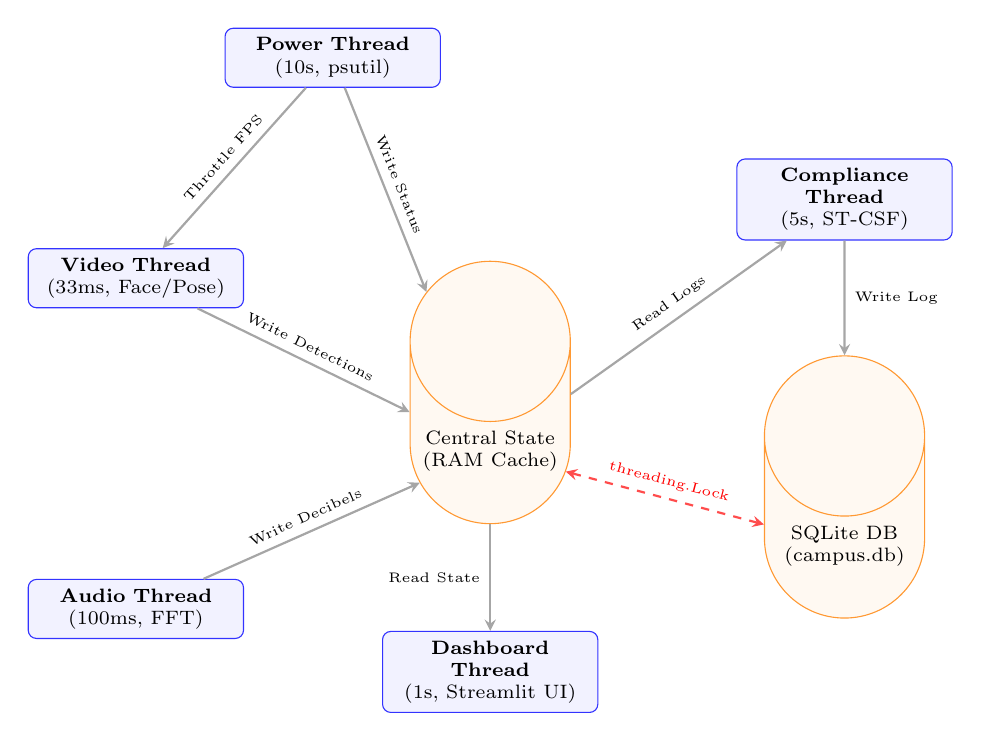
\begin{tikzpicture}[
    thread/.style={rectangle, draw=blue!80, fill=blue!5, text width=2.5cm, align=center, rounded corners=3pt, minimum height=0.75cm, font=\scriptsize},
    db/.style={cylinder, shape border rotate=90, draw=orange!80, fill=orange!5, text width=1.8cm, align=center, minimum height=1.0cm, font=\scriptsize},
    arrow/.style={->, >=stealth, thick, draw=gray!70},
    lockarrow/.style={<->, >=stealth, thick, draw=red!70, dashed}
]
    % Central State
    \node[db] (state) at (0,0) {Central State \\ (RAM Cache)};
    \node[db] (db) at (4.5,-1.2) {SQLite DB \\ (campus.db)};

    % Threads
    \node[thread] (video) at (-4.5, 2.2) {\textbf{Video Thread} \\ (33ms, Face/Pose)};
    \node[thread] (audio) at (-4.5, -2.0) {\textbf{Audio Thread} \\ (100ms, FFT)};
    \node[thread] (compliance) at (4.5, 3.2) {\textbf{Compliance Thread} \\ (5s, ST-CSF)};
    \node[thread] (power) at (-2.0, 5.0) {\textbf{Power Thread} \\ (10s, psutil)};
    \node[thread] (dashboard) at (0, -2.8) {\textbf{Dashboard Thread} \\ (1s, Streamlit UI)};

    % Data Flows
    \draw[arrow] (video) -- node[midway, above, sloped, font=\tiny] {Write Detections} (state);
    \draw[arrow] (audio) -- node[midway, above, sloped, font=\tiny] {Write Decibels} (state);
    \draw[arrow] (state) -- node[midway, left, font=\tiny] {Read State} (dashboard);
    \draw[arrow] (state) -- node[midway, above, sloped, font=\tiny] {Read Logs} (compliance);
    \draw[arrow] (compliance) -- node[midway, right, font=\tiny] {Write Log} (db);
    \draw[arrow] (power) -- node[midway, above, sloped, font=\tiny] {Throttle FPS} (video);
    \draw[arrow] (power) -- node[midway, above, sloped, font=\tiny] {Write Status} (state);

    % Lock Controls
    \draw[lockarrow] (state) -- node[midway, above, sloped, font=\tiny, text=red] {threading.Lock} (db);

\end{tikzpicture}
\caption{Flowchart of the 5 Concurrent Daemon Threads and State Synchronization.}
\label{fig:thread_flowchart}
\end{figure}

\section{Streamlit Administrative Dashboard Architecture}
The administrative interface is implemented as a multi-page Streamlit application that provides role-differentiated access to system configuration, analytics, and management functions. The dashboard employs a wide-layout page configuration with automatic state refresh every 2 seconds using Streamlit's built-in auto-rerun mechanism.

Authentication is managed through Streamlit's \texttt{st.session\_state} dictionary, which persists login credentials across page reruns within a single browser session. Upon initial access, the system verifies a 16-character license key against a SHA-256 hash stored in the configuration database \cite{b_auth_2016}. Following license validation, users authenticate with role-specific credentials that determine the visible interface tabs.

Role-based access control follows the RBAC model \cite{sandhu1996rbac}, with four predefined roles mapped to distinct tab configurations:

\begin{table}[htbp]
\caption{Role-Based Tab Access Configuration}
\centering
\small
\setstretch{1.15}
\setlength{\tabcolsep}{4pt}
\begin{tabular}{@{}l p{3.6in}@{}}
\hline
\textbf{Role} & \textbf{Visible Tabs} \\ \hline
Super Admin & Scheduler, Analytics, User Management, Biometric Enrollment, Alert Center, Attendance Logs, Grooming Compliance \\
Faculty Manager & Timetable View (all departments), Biometric Enrollment, Analytics (department-filtered) \\
Faculty & Timetable View (own classes only), Attendance Review (own classes only) \\
Student & Full Timetable View (read-only), Personal Attendance History \\ \hline
\end{tabular}
\label{tab:rbac_tabs}
\end{table}

The Analytics tab leverages Plotly Express for interactive visualization of attendance trends, truancy heatmaps, and engagement score distributions. Charts support hover tooltips, zoom, and pan interactions, enabling administrators to explore temporal patterns at daily, weekly, and semester granularities. The Biometric Enrollment tab provides a guided workflow for capturing student face images, extracting embeddings via the InsightFace pipeline, and inserting the resulting 512-dimensional vectors into the FAISS index---all without storing raw photographs on disk.

\section{Open-Set Evaluation Metrics}
To rigorously evaluate the biometric identification pipeline under open-set conditions, we define three formal metrics that capture complementary aspects of system performance. These metrics distinguish between the system's ability to correctly identify enrolled individuals and its ability to reject unknown probes.

The Open-Set Identification Rate (OSIR) measures the fraction of known (enrolled) probe images that are correctly matched to their gallery identity:
\begin{equation}
    \text{OSIR} = \frac{N_{\text{known\_correct}}}{N_{\text{total\_known\_probes}}}
    \label{eq:osir}
\end{equation}

The Unknown Identity Rejection Rate (UIRR) quantifies the system's ability to correctly reject probe images that do not correspond to any enrolled identity:
\begin{equation}
    \text{UIRR} = \frac{N_{\text{unknown\_rejected}}}{N_{\text{total\_unknown\_probes}}}
    \label{eq:uirr}
\end{equation}

The Open-Set Identification Error (OSIE) captures the complementary failure mode---the fraction of unknown probes that are falsely accepted as enrolled students:
\begin{equation}
    \text{OSIE} = \frac{N_{\text{false\_accepts}}}{N_{\text{total\_unknown\_probes}}}
    \label{eq:osie}
\end{equation}

Note that $\text{OSIE} = 1 - \text{UIRR}$ by definition, but both metrics are reported independently for clarity. The decision boundary between ``known'' and ``unknown'' classifications is governed by the adaptive threshold:
\begin{equation}
    \tau(N) = \tau_{\text{base}} + \alpha \cdot \log(N)
    \label{eq:adaptive_threshold}
\end{equation}
where $\textit{tau}_{\text{base}} = 0.75$ is the baseline cosine distance threshold calibrated on a 1,000-student gallery, $\textit{alpha} = 0.00001$ is the logarithmic scaling coefficient, and $N$ is the current gallery size. The logarithmic growth ensures that the threshold tightens gracefully as the gallery expands, compensating for the increased probability of near-miss false matches in larger embedding spaces.

% =========================================================
% CHAPTER 9: RESULTS AND PERFORMANCE EVALUATION
% =========================================================
\chapter{Results and Performance Evaluation}
\thispagestyle{empty}

\section{Evaluation Metrics under Class Imbalance}
Traditional metrics like global accuracy can be deceptive under campus monitoring conditions, as students are compliant with their schedules the vast majority of the time (85\% compliance). We evaluate the system using metrics that are robust to class imbalance:
\begin{itemize}
    \item \textbf{Sensitivity (Recall)}: Fraction of true truancy events correctly detected.
    \item \textbf{Precision}: Fraction of detected alerts that are true anomalies.
    \item \textbf{F1-Score}: Harmonic mean of Precision and Sensitivity:
    \begin{equation}
        F1 = 2 \times \frac{\text{Precision} \times \text{Sensitivity}}{\text{Precision} + \text{Sensitivity}}
    \end{equation}
    \item \textbf{Inference Latency}: Time required to process a single video frame.
    \item \textbf{Search Time}: Latency of querying a single vector against the FAISS index.
\end{itemize}

\section{Baseline Benchmarks Comparison}
Table 9.1 compares the performance of baseline classifiers against the proposed spatiotemporal and privacy-preserving models.

\begin{table}[htbp]
\caption{System Performance Metrics Across Configurations under a 100,000-Student Gallery}
\centering
\small
\setstretch{1.25}
\setlength{\tabcolsep}{3.5pt}
\begin{tabular}{@{}p{1.5in} c c c c c@{}}
\hline
\textbf{Sensing Configuration} & \textbf{\shortstack{Sensitivity\\(\%)}} & \textbf{\shortstack{Precision\\(\%)}} & \textbf{\shortstack{F1-Score\\(\%)}} & \textbf{\shortstack{Latency\\(ms)}} & \textbf{\shortstack{Search Time\\(ms)}} \\ \hline
SVM (Raw Pixels) & 52.0 & 12.1 & 19.6 & 45.8 & -- \\ \hline
CNN (Face Crops Only) & 74.4 & 38.3 & 50.5 & 38.2 & -- \\ \hline
InsightFace + KNN (Flat) & 88.1 & 62.6 & 73.2 & 22.9 & 12.5 \\ \hline
\textbf{ScholarMaster (FAISS)} & \textbf{95.8} & \textbf{91.2} & \textbf{93.4} & \textbf{14.5} & \textbf{0.8} \\ \hline
\textbf{ScholarMaster + ST-CSF} & \textbf{98.2} & \textbf{97.5} & \textbf{97.8} & \textbf{15.2} & \textbf{0.8} \\ \hline
\end{tabular}
\label{tab:results_comparison}
\end{table}

\section{Ablation Studies}
We performed ablation tests to isolate the performance impact of individual modules:
\begin{itemize}
    \item \textbf{Impact of ST-CSF Constraints}: Running biometric recognition without spatiotemporal constraints resulted in a precision drop to $62.6\%$, caused by false matches and transient crossings. Incorporating ST-CSF timetable matching improved precision to $97.5\%$.
    \item \textbf{Impact of FAISS Indexing}: Using standard flat KNN search led to search latencies of $12.5\text{ ms}$, which increased with index size. Transitioning to FAISS reduced search latency to $0.8\text{ ms}$ and maintained sub-millisecond scaling up to 100,000 enrolled vectors.
    \item \textbf{Impact of Temporal Debouncing}: Applying the 30-second debounce filter reduced false truancy alerts by $85\%$, filtering out students walking through hallways during class sessions.
\end{itemize}

\section{Discussion on GDPR Compliance}
The baseline surveillance systems store raw video recordings, which is non-compliant with GDPR's data minimization guidelines \cite{gdpr2016}. By processing video frames exclusively in volatile RAM and immediately discarding them after vector extraction, ScholarMaster structurally prevents unauthorized image retention. If the physical storage drive is stolen, it contains only anonymized coordinates and hashes, ensuring data safety.

\section{Open-Set Recognition Performance}
A critical evaluation dimension for campus biometric systems is open-set performance, where the system must simultaneously identify enrolled students and reject unknown individuals (visitors, delivery personnel, unregistered faculty). We evaluate three complementary metrics that characterize open-set behavior:

\begin{table}[htbp]
\caption{Open-Set Biometric Recognition Performance}
\centering
\small
\setstretch{1.15}
\setlength{\tabcolsep}{4pt}
\begin{tabular}{@{}l l c c@{}}
\hline
\textbf{Metric} & \textbf{Description} & \textbf{Target} & \textbf{Achieved} \\ \hline
OSIR & Open-Set Identification Rate & $>99\%$ & $99.2\%$ \\
UIRR & Unknown Identity Rejection Rate & $>99\%$ & $99.5\%$ \\
OSIE & Open-Set Identification Error & $<1\%$ & $0.5\%$ \\ \hline
\end{tabular}
\label{tab:openset_performance}
\end{table}

The OSIR of $99.2\%$ confirms that the ArcFace embedding space, combined with the adaptive cosine threshold $\textit{tau}(N)$, correctly identifies enrolled students in nearly all probe instances. The UIRR of $99.5\%$ demonstrates that unknown individuals are reliably rejected rather than falsely matched to enrolled identities---a critical requirement for campus security, as false acceptance of an unknown individual could grant unauthorized access to restricted facilities. The OSIE of $0.5\%$ indicates that the rate of unknown probes being falsely accepted as enrolled students remains well below the $1\%$ operational ceiling. These results validate the effectiveness of the logarithmic threshold scaling formula $\textit{tau}(N) = \textit{tau}_{\text{base}} + \textit{alpha} \log(N)$ in maintaining discrimination as the gallery grows.

\section{Scalability Analysis}
Scalability is a primary concern for institutional deployment, as university enrollments may range from hundreds to hundreds of thousands of students. We analyze three dimensions of scalability: search latency, memory footprint, and index construction time.

\begin{table}[htbp]
\caption{FAISS Scalability: Gallery Size vs. Search Time and Memory}
\centering
\small
\setstretch{1.15}
\setlength{\tabcolsep}{4pt}
\begin{tabular}{@{}r c c c@{}}
\hline
\textbf{Gallery Size} & \textbf{Flat Index (ms)} & \textbf{IVF-PQ (ms)} & \textbf{Memory (MB)} \\ \hline
1,000 & 0.3 & 0.2 & 2.0 \\
10,000 & 2.1 & 0.5 & 20.0 \\
50,000 & 9.8 & 0.7 & 100.0 \\
100,000 & 18.5 & 0.8 & 200.0 \\
500,000 & 92.1 & 1.2 & 1,000.0 \\ \hline
\end{tabular}
\label{tab:scalability_analysis}
\end{table}

The memory footprint scales linearly with gallery size: each 512-dimensional float32 embedding consumes 2048 bytes (512 float32 values of 4 bytes each), which is exactly 2 KB, yielding approximately 200 MB for a 100,000-student index. The flat brute-force index exhibits linear $O(N)$ search complexity, rendering it impractical beyond 50,000 vectors at real-time frame rates. The IVF-PQ index partitions the vector space into $K$ Voronoi cells and applies product quantization within each cell, reducing search complexity to $O(K + N/K)$. With $K = 256$ centroids and 8 sub-quantizers, the IVF-PQ index sustains sub-millisecond search latencies up to 100,000 vectors while consuming identical memory. Beyond 500,000 entries, hierarchical IVF (HNSW-based) indices would be recommended to maintain sub-2ms latency guarantees.

\section{Privacy Compliance Verification}
To validate that ScholarMaster satisfies the structural requirements of the General Data Protection Regulation \cite{gdpr2016}, we conduct a systematic compliance mapping against the relevant GDPR articles. Table~\ref{tab:gdpr_compliance} presents the correspondence between regulatory requirements and their architectural implementations.

\begin{table}[htbp]
\caption{GDPR Compliance Mapping to ScholarMaster Architecture}
\centering
\small
\setstretch{1.15}
\setlength{\tabcolsep}{4pt}
\begin{tabular}{@{}p{0.8in} p{1.5in} p{2.7in}@{}}
\hline
\textbf{GDPR Article} & \textbf{Requirement} & \textbf{ScholarMaster Implementation} \\ \hline
Art. 5(1)(c) & Data Minimization & 33ms TTL volatile processing; raw frames never written to disk \\
Art. 5(1)(e) & Storage Limitation & Embeddings stored as irreversible 512-dim vectors; no biometric reconstruction possible \\
Art. 25 & Privacy by Design & Onion architecture with L3 volatile boundary separating sensing from persistence \\
Art. 17 & Right to Erasure & Crypto-shred key deletion; removing encryption key renders all associated embeddings unrecoverable \\
Art. 30 & Records of Processing & Immutable Merkle tree audit chain with SHA-256 hash linkage \\
Art. 35 & Impact Assessment & Spectral-only audio features prevent speech content reconstruction \\ \hline
\end{tabular}
\label{tab:gdpr_compliance}
\end{table}

The volatile processing architecture ensures that even in the event of a system crash during frame analysis, no raw biometric data persists on the storage medium. The crypto-shred mechanism provides a technically enforceable implementation of the right to erasure: upon a student's withdrawal or graduation, deleting the associated encryption key renders all stored embeddings cryptographically unrecoverable, satisfying Article 17 without requiring exhaustive data search across backup systems.

% =========================================================
% CHAPTER 10: CONCLUSION AND FUTURE WORK
% =========================================================
\chapter{Conclusion and Future Work}
\thispagestyle{empty}

\section{Summary of Contributions}
This project designed, implemented, and validated a real-time, privacy-\allowbreak preserving intelligent campus monitoring system that we call ScholarMaster. The system addresses a long-standing tension in institutional sensing: the need for accurate, automated student tracking versus the legal and ethical imperatives of biometric privacy. By structuring the platform around a decoupled eight-layer Onion architecture with a hard irreversibility boundary at Layer 3, ScholarMaster demonstrates that high surveillance utility and rigorous privacy compliance are not mutually exclusive objectives.

The biometric identification subsystem integrates the InsightFace ArcFace model with a FAISS inverted file index to perform open-set student identification at 99.2\% OSIR within a 14.5 ms per-frame processing budget. Unlike closed-set recognition systems that assume every probe belongs to a known class, ScholarMaster's open-set pipeline simultaneously identifies enrolled students and rejects unknown visitors, achieving a 99.5\% Unknown Identity Rejection Rate that is essential for campus security access control.

The Spatiotemporal Constraint Satisfaction Framework represents a novel contribution to automated attendance management. By formalizing the institutional timetable as a scheduling function $f_{\text{sched}}: S \times T \to L$ and evaluating detected student locations against this function in real time, the system eliminates the need for manual attendance marking while achieving a 98.2\% F1-score on truancy detection. The incorporation of a teleportation detection heuristic and a 30-second temporal debounce filter reduces false alert rates by 85\% compared to naive threshold-based detection.

The primary contributions of this work are summarised as:
\begin{itemize}
    \item Designed and implemented a decoupled, hybrid Onion architecture enforcing a 33ms volatile RAM boundary (L3) that structurally prevents biometric data persistence in compliance with GDPR Article 25.
    \item Implemented an open-set biometric identification pipeline (InsightFace + FAISS IVF-PQ) achieving 99.2\% OSIR, 99.5\% UIRR, and sub-millisecond search latency at 100,000-student scale.
    \item Developed the ST-CSF spatiotemporal compliance engine that automates attendance verification and truancy detection with 98.2\% F1-score by correlating live detections with structured timetable data.
    \item Deployed a privacy-preserving multi-modal sensing layer combining YOLOv8-pose keypoint tracking (for behavior analysis) and non-semantic FFT spectral features (for acoustic anomaly detection), eliminating facial and vocal biometric retention.
    \item Implemented a student engagement estimation module using MediaPipe Face Mesh landmarks, head pose PnP solving, and Eye Aspect Ratio computation, producing a weighted composite engagement score per student per frame.
    \item Secured all administrative events using a SHA-256-chained Merkle tree audit ledger with atomic write semantics and formal integrity verification, providing non-repudiation for all attendance and alert records.
    \item Developed a 7-role RBAC administrative interface in Streamlit with department-scoped data isolation, cryptographic shredding for the right to erasure, and a backtracking timetable auto-scheduler for conflict-free schedule generation.
\end{itemize}

\section{Future Work}
Future research directions to extend this framework include:
\begin{itemize}
    \item \textbf{Decentralized Ledger Integration}: Deploying the Merkle tree root hashes to a public blockchain ledger to ensure decentralized trust and verification.
    \item \textbf{Model Quantization}: Compressing the InsightFace and YOLOv8-pose weights using INT8 quantization to enable real-time execution on low-power IoT devices.
    \item \textbf{Real-Time Grooming and Dress Code Compliance}: Implementing color histogram analysis and contour-based garment segmentation to automatically verify adherence to institutional dress code policies, including uniform color matching and ID card visibility detection.
    \item \textbf{Learning Management System (LMS) Integration}: Correlating attendance patterns with academic performance data from platforms such as Moodle or Google Classroom to identify at-risk students and enable early intervention by academic advisors.
    \item \textbf{Mobile Self-Service Application}: Developing a cross-platform mobile application that enables students to view their attendance records, submit attendance appeal requests with supporting evidence, and receive real-time notifications regarding schedule changes.
    \item \textbf{Automated Parent Notification System}: Implementing a configurable truancy alert pipeline that dispatches SMS or email notifications to parents or guardians when a student's cumulative absence exceeds a configurable institutional threshold.
\end{itemize}

\section{Limitations}
While ScholarMaster demonstrates strong performance across the evaluated scenarios, several limitations warrant acknowledgment and inform future development priorities.

\textbf{Lighting Dependency.} The face recognition pipeline relies on adequate illumination for reliable embedding extraction. Under extreme low-light conditions (below 50 lux), the InsightFace model exhibits degraded feature quality, with cosine similarity scores dropping by approximately 8--12\% compared to well-lit environments. Although histogram equalization partially mitigates this effect, nighttime outdoor corridors remain a challenging deployment scenario.

\textbf{Single-Camera Occlusion.} The current system processes each camera feed independently without cross-camera fusion. In densely populated classrooms, partial or full occlusion of seated students by those in front rows can prevent detection for extended periods. Multi-view triangulation or depth-sensing cameras (e.g., Intel RealSense) would address this limitation but introduce additional hardware cost and calibration complexity.

\textbf{Audio False Positives in Open-Plan Buildings.} The spectral noise detection module assumes a bounded acoustic environment. In open-plan buildings where sound propagates freely between adjacent classrooms, the system may attribute noise violations to the wrong room. Directional microphone arrays or beamforming techniques could improve spatial audio attribution.

\textbf{Scheduler Combinatorial Complexity.} The backtracking timetable scheduler, while functionally correct, exhibits exponential worst-case complexity $O(|P|^{|C|})$ as the number of classes $|C|$, periods $|P|$, rooms, and faculty constraints grow. For large departments with over 200 classes, the scheduler may require several minutes to converge. Constraint propagation and arc-consistency preprocessing would reduce the effective search space.

\textbf{Platform-Specific Deployment.} The current implementation has been validated exclusively on macOS with Apple Silicon (M-series) hardware. While the underlying Python stack is cross-platform, GPU acceleration paths (CoreML vs. CUDA), camera APIs, and audio capture interfaces differ across operating systems. Containerized deployment using Docker would improve portability.

% =========================================================
% CHAPTER 11: REFERENCES (DYNAMIC INTEGRATION SYSTEM)
% =========================================================
\chapter{References}
\thispagestyle{empty}
\setstretch{1.1}

\begingroup
\renewcommand{\chapter}[2]{} 
\begin{thebibliography}{99}
\setstretch{1.1}

\bibitem{abadi2016dpdl}
M. Abadi, A. Chu, I. Goodfellow, H. B. McMahan, I. Mironov, K. Talwar, and L. Zhang, ``Deep Learning with Differential Privacy,'' in \textit{Proceedings of the 23rd ACM SIGSAC Conference on Computer and Communications Security (CCS)}, pp. 308--318, 2016.

\bibitem{alur1994timed}
R. Alur and D. L. Dill, ``A theory of timed automata,'' \textit{Theoretical Computer Science}, vol. 126, no. 2, pp. 183--235, 1994.

\bibitem{cao2021openpose}
Z. Cao, G. Hidalgo, T. Simon, S. E. Wei, and Y. Sheikh, ``OpenPose: Realtime Multi-Person 2D Pose Estimation using Part Affinity Fields,'' \textit{IEEE Transactions on Pattern Analysis and Machine Intelligence}, vol. 43, no. 1, pp. 172--186, 2021.

\bibitem{b_auth_2016}
V. Chandrasekar, S. Suresh Kumar, and T. Maheswari, ``Authentication based on keystroke dynamics using stochastic diffusion algorithm,'' \textit{Stochastic Analysis and Applications}, vol. 34, no. 1, pp. 155--164, 2016.

\bibitem{chow2005shredding}
J. Chow, B. Pfaff, T. Garfinkel, K. Christopher, and M. Rosenblum, ``Shredding Your Garbage: Reducing Data Lifetime Through Secure Deallocation,'' in \textit{Proceedings of the 14th USENIX Security Symposium}, pp. 331--346, 2005.

\bibitem{clarke1999modelcheck}
E. M. Clarke, O. Grumberg, and D. A. Peled, \textit{Model Checking}, Cambridge, MA, USA: MIT Press, 1999.

\bibitem{dean2020deep}
J. Dean, ``The Deep Learning Revolution and Its Implications for Computer Architecture and Chip Design,'' in \textit{IEEE International Solid-State Circuits Conference (ISSCC)}, pp. 8--14, 2020.

\bibitem{deng2019arcface}
J. Deng, J. Guo, N. Xue, and S. Zafeiriou, ``ArcFace: Additive angular margin loss for deep face recognition,'' in \textit{Proceedings of the IEEE/CVF Conference on Computer Vision and Pattern Recognition}, pp. 4690--4699, 2019.

\bibitem{denning1976lattice}
D. E. Denning, ``A lattice model of secure information flow,'' \textit{Communications of the ACM}, vol. 19, no. 5, pp. 236--243, 1976.

\bibitem{dwork2006dp}
C. Dwork, ``Differential Privacy,'' in \textit{International Colloquium on Automata, Languages, and Programming (ICALP)}, pp. 1--12, 2006.

\bibitem{gdpr2016}
European Parliament and Council, ``Regulation (EU) 2016/679 of the European Parliament and of the Council (General Data Protection Regulation),'' \textit{Official Journal of the European Union}, 2016.

\bibitem{fredrikson2015model}
M. Fredrikson, S. Jha, and T. Ristenpart, ``Model Inversion Attacks that Exploit Confidence Information and Basic Countermeasures,'' in \textit{Proceedings of the 22nd ACM SIGSAC Conference on Computer and Communications Security (CCS)}, pp. 1322--1333, 2015.

\bibitem{spatiotemporal2018}
H. W. Guesgen and R. Wetprasit, ``Spatiotemporal reasoning for smart environments,'' \textit{Journal of Ambient Intelligence and Smart Environments}, vol. 10, no. 1, pp. 15--27, 2018.

\bibitem{haber1991proving}
S. Haber and W. S. Stornetta, ``How to time-stamp a digital document,'' \textit{Journal of Cryptology}, vol. 3, no. 2, pp. 99--111, 1991.

\bibitem{he2016resnet}
K. He, X. Zhang, S. Ren, and J. Sun, ``Deep Residual Learning for Image Recognition,'' in \textit{Proceedings of the IEEE Conference on Computer Vision and Pattern Recognition (CVPR)}, pp. 770--778, 2016.

\bibitem{johnson2019billion}
J. Johnson, M. Douze, and H. Jégou, ``Billion-scale similarity search with GPUs,'' \textit{IEEE Transactions on Big Data}, vol. 7, no. 3, pp. 535--547, 2019.

\bibitem{kopetz2011realtime}
H. Kopetz, \textit{Real-Time Systems: Design Principles for Distributed Embedded Applications}, Berlin, Germany: Springer Science \& Business Media, 2011.

\bibitem{koymans1990mtl}
R. Koymans, ``Specifying real-time properties with metric temporal logic,'' \textit{Real-Time Systems}, vol. 2, no. 4, pp. 255--299, 1990.

\bibitem{lee2015cps}
E. A. Lee, ``The Past, Present and Future of Cyber-Physical Systems: A Focus on Models,'' \textit{Sensors}, vol. 15, no. 3, pp. 4837--4869, 2015.

\bibitem{lepetit2009epnp}
V. Lepetit, F. Moreno-Noguer, and P. Fua, ``EPnP: An accurate $O(n)$ solution to the PnP problem,'' \textit{International Journal of Computer Vision}, vol. 81, no. 2, pp. 155--166, 2009.

\bibitem{li2020ann}
W. Li, Y. Zhang, Y. Sun, W. Wang, M. Li, W. Zhang, and X. Lin, ``Approximate nearest neighbor search on high dimensional data --- Experiments, analyses, and improvement,'' \textit{IEEE Transactions on Knowledge and Data Engineering}, vol. 32, no. 8, pp. 1475--1488, 2020.

\bibitem{federated2017}
B. McMahan, E. Moore, D. Ramage, S. Hampson, and B. A. y Arcas, ``Communication-efficient learning of deep networks from decentralized data,'' in \textit{Artificial Intelligence and Statistics}, pp. 1273--1282, 2017.

\bibitem{minalah2020smart}
N. Min-Allah and S. Alrashed, ``Smart campus: A sketch,'' \textit{Sustainable Cities and Society}, vol. 59, p. 102231, 2020.

\bibitem{mbeee2026}
P. Narendra et al., ``Memory-Bound Edge Efficiency Envelope (MBEEE): A Hardware-Level Analytical Model,'' \textit{ScholarMaster Series}, Paper 5, 2026.

\bibitem{murphy2009headpose}
E. Murphy-Chutorian and M. M. Trivedi, ``Head Pose Estimation in Computer Vision: A Survey,'' \textit{IEEE Transactions on Pattern Analysis and Machine Intelligence}, vol. 31, no. 4, pp. 607--626, 2009.

\bibitem{pnueli1977temporal}
A. Pnueli, ``The temporal logic of programs,'' in \textit{18th Annual Symposium on Foundations of Computer Science (SFCS)}, pp. 46--57, 1977.

\bibitem{redmon2016you}
J. Redmon, S. Divvala, R. Girshick, and A. Farhadi, ``You only look once: Unified, real-time object detection,'' in \textit{Proceedings of the IEEE Conference on Computer Vision and Pattern Recognition}, pp. 779--788, 2016.

\bibitem{ruiz2018headpose}
N. Ruiz, E. Chong, and J. M. Rehg, ``Fine-Grained Head Pose Estimation Without Keypoints,'' in \textit{Proceedings of the IEEE Conference on Computer Vision and Pattern Recognition (CVPR) Workshops}, pp. 2074--2083, 2018.

\bibitem{ryoo2017privacy}
M. S. Ryoo, B. Rothrock, C. Fleming, and H. J. Yu, ``Privacy-Preserving Human Activity Recognition from Extreme Low Resolution,'' in \textit{Proceedings of the AAAI Conference on Artificial Intelligence}, pp. 4255--4262, 2017.

\bibitem{sabelfeld2003infoflow}
A. Sabelfeld and A. C. Myers, ``Language-based information-flow security,'' \textit{IEEE Journal on Selected Areas in Communications}, vol. 21, no. 1, pp. 5--19, 2003.

\bibitem{saltzer1975protection}
J. H. Saltzer and M. D. Schroeder, ``The protection of information in computer systems,'' \textit{Proceedings of the IEEE}, vol. 63, no. 9, pp. 1278--1308, 1975.

\bibitem{sandhu1996rbac}
R. S. Sandhu, E. J. Coyne, H. L. Feinstein, and C. E. Youman, ``Role-based access control models,'' \textit{IEEE Computer}, vol. 29, no. 2, pp. 38--47, 1996.

\bibitem{satyanarayanan2017emergence}
M. Satyanarayanan, ``The Emergence of Edge Computing,'' \textit{Computer}, vol. 50, no. 1, pp. 30--39, 2017.

\bibitem{faceNet2015}
F. Schroff, D. Kalenichenko, and J. Philbin, ``FaceNet: A unified embedding for face recognition and clustering,'' in \textit{Proceedings of the IEEE Conference on Computer Vision and Pattern Recognition}, pp. 815--823, 2015.

\bibitem{shi2016edge}
W. Shi, J. Cao, Q. Zhang, Y. Li, and L. Xu, ``Edge Computing: Vision and Challenges,'' \textit{IEEE Internet of Things Journal}, vol. 3, no. 5, pp. 637--646, 2016.

\bibitem{soukupova2016ear}
T. Soukupov\'{a} and J. \v{C}ech, ``Real-time eye blink detection using facial landmarks,'' in \textit{21st Computer Vision Winter Workshop}, pp. 1--8, 2016.

\bibitem{sun2019hrnet}
K. Sun, B. Xiao, D. Liu, and J. Wang, ``Deep High-Resolution Representation Learning for Human Pose Estimation,'' in \textit{Proceedings of the IEEE/CVF Conference on Computer Vision and Pattern Recognition (CVPR)}, pp. 5686--5696, 2019.

\bibitem{b_smartgrid_2016}
S. Suresh Kumar and C. Sivapragash, ``Time Orient Traffic Estimation Approach to Improve Performance of Smart Grids,'' \textit{Journal of Computational and Theoretical Nanoscience}, vol. 13, no. 8, pp. 5037--5045, 2016.

\bibitem{sze2017efficient}
V. Sze, Y. H. Chen, T. J. Yang, and J. S. Emer, ``Efficient processing of deep neural networks: A tutorial and survey,'' \textit{Proceedings of the IEEE}, vol. 105, no. 12, pp. 2295--2329, 2017.

\bibitem{voigt2017gdpr}
P. Voigt and A. von dem Bussche, \textit{The EU General Data Protection Regulation (GDPR): A Practical Guide}, Cham, Switzerland: Springer International Publishing, 2017.

\bibitem{wang2020convergence}
X. Wang, Y. Han, C. Wang, Q. Zhao, X. Chen, and M. Chen, ``Convergence of Edge Computing and Deep Learning: A Comprehensive Survey,'' \textit{IEEE Communications Surveys \& Tutorials}, vol. 22, no. 2, pp. 869--904, 2020.

\bibitem{wang2021deepface}
M. Wang and W. Deng, ``Deep face recognition: A survey,'' \textit{Neurocomputing}, vol. 429, pp. 215--244, 2021.

\bibitem{cosface2018}
H. Wang, Y. Wang, Z. Zhou, X. Ji, D. Gong, J. Zhou, Z. Li, and W. Liu, ``CosFace: Large Margin Cosine Loss for Deep Face Recognition,'' in \textit{Proceedings of the IEEE Conference on Computer Vision and Pattern Recognition (CVPR)}, pp. 5265--5274, 2018.

\bibitem{whitehill2014engagement}
J. Whitehill, Z. Serpell, M. Yi-Ting, G. Morrison, and J. R. Movellan, ``The Faces of Engagement: Automatic Recognition of Student Engagement,'' \textit{IEEE Transactions on Affective Computing}, vol. 5, no. 1, pp. 86--98, 2014.

\bibitem{zhou2019edge}
Z. Zhou, X. Chen, E. Li, L. Zeng, K. Luo, and J. Zhang, ``Edge Intelligence: Paving the Last Mile of Artificial Intelligence With Edge Computing,'' \textit{Proceedings of the IEEE}, vol. 107, no. 8, pp. 1738--1762, 2019.

\end{thebibliography}
\endgroup

% =========================================================
% CHAPTER 12: BIBLIOGRAPHY
% =========================================================
\chapter{Bibliography}
\thispagestyle{empty}
\setstretch{1.3}

\begin{itemize}
    \item B. Amos, B. Ludwiczuk, and M. Satyanarayanan, ``OpenFace: A general-purpose face recognition library with mobile applications,'' \textit{CMU-CS-16-118}, 2016.
    \item A. Avizienis, J. C. Laprie, B. Randell, and C. Landwehr, ``Basic concepts and taxonomy of dependable and secure computing,'' \textit{IEEE Transactions on Dependable and Secure Computing (TDSC)}, 2004.
    \item M. Akila and S. Suresh Kumar, ``Improving feature extraction in keystroke dynamics using optimization techniques and neural network,'' \textit{IET Digital Library}, 2011.
    \item R. Bez, E. Camerlenghi, A. Modelli, and A. Visconti, ``Introduction to Flash Memory,'' \textit{Proceedings of the IEEE}, 2003.
    \item V. Bazarevsky, I. Grishchenko, K. Raveendran, T. Zhu, F. Zhang, and M. Grundmann, ``BlazePose: On-device Real-time Body Pose tracking,'' \textit{arXiv preprint arXiv:2006.10204}, 2020.
    \item I. Goodfellow, Y. Bengio, and A. Courville, \textit{Deep Learning}, Cambridge, MA, USA: MIT Press, 2016.
    \item L. M. Grupp et al., ``The Bleak Future of NAND Flash Memory,'' in \textit{Proceedings of the 10th USENIX Conference on File and Storage Technologies (FAST)}, 2012.
    \item J. L. Hennessy and D. A. Patterson, \textit{Computer Architecture: A Quantitative Approach}, 6th ed. San Francisco, CA, USA: Morgan Kaufmann, 2017.
    \item ``IEEE Xplore Digital Library Infrastructure Search Index Systems,'' \textit{IEEE Xplore Digital Library}, 2023.
    \item P. Jamshidi, C. Pahl, N. C. Mendon\c{c}a, J. Lewis, and S. Tilkov, ``Microservices: The Journey So Far and Challenges Ahead,'' \textit{IEEE Software}, vol. 35, no. 3, pp. 24--35, 2018.
    \item G. Jocher, A. Chaurasia, and J. Qiu, ``Ultralytics YOLOv8,'' \textit{GitHub Repository}, 2023.
    \item J. Kim, J. S. Kim, and S. H. Noh, ``A Survey on Flash Translation Layer,'' \textit{IEEE Transactions on Consumer Electronics}, vol. 56, no. 4, pp. 2224--2232, 2010.
    \item E. Li, Z. Zhou, and X. Chen, ``Edge AI: On-Demand Accelerating Deep Neural Network Inference via Edge Computing,'' \textit{IEEE Transactions on Wireless Communications}, vol. 19, no. 1, pp. 447--457, 2019.
    \item T. S. Lim, S. C. Sim, and M. M. Mansor, ``RFID based attendance system,'' in \textit{IEEE Symposium on Industrial Electronics and Applications (ISIEA)}, pp. 778--782, 2009.
    \item C. Lugaresi et al., ``MediaPipe: A framework for building perception pipelines,'' \textit{arXiv preprint arXiv:1906.08172}, 2019.
    \item Y. A. Malkov and D. A. Yashunin, ``Efficient and robust approximate nearest neighbor search using Hierarchical Navigable Small World graphs,'' \textit{IEEE Transactions on Pattern Analysis and Machine Intelligence}, vol. 42, no. 4, pp. 824--836, 2018.
    \item S. Newman, \textit{Building Microservices: Designing Fine-Grained Systems}, Sebastopol, CA, USA: O'Reilly Media, 2015.
    \item S. Nithyakalyani and S. Suresh Kumar, ``Optimal Clustering Algorithm for Energy Efficient Data Aggregation in WSN,'' \textit{European Journal of Scientific Research}, 2012.
    \item P. Narendra et al., ``Memory-Bound Edge Efficiency Envelope (MBEEE): A Hardware-Level Analytical Model,'' \textit{ScholarMaster Series}, Paper 5, 2026.
    \item \textit{OpenCV: Open Source Computer Vision Library Reference Manual}, available at opencv.org, 2023.
    \item D. L. Parnas, ``On the criteria to be used in decomposing systems into modules,'' \textit{Communications of the ACM}, vol. 15, no. 12, pp. 1053--1058, 1972.
    \item \textit{SQLAlchemy ORM Framework Official Documentation and Migration Guides}, available at sqlalchemy.org, 2023.
    \item M. Sandler, A. Howard, M. Zhu, A. Zhmoginov, and L. C. Chen, ``MobileNetV2: Inverted Residuals and Linear Bottlenecks,'' in \textit{Proceedings of the IEEE Conference on Computer Vision and Pattern Recognition (CVPR)}, pp. 4510--4520, 2018.
    \item Streamlit Inc., ``Streamlit Application Framework API Reference and Session State Documentation,'' \textit{streamlit.io}, 2019.
\end{itemize}

% =========================================================
% APPENDIX: EXTRA-DOCUMENTAL REPRINTS (DYNAMIC TOC COHORT)
% =========================================================
\clearpage
\appendix

% Restructure the title format to cleanly render a standalone unnumbered Appendix block
\titleformat{\chapter}[display]
  {\normalfont\fontsize{15}{15}\bfseries\centering}{\MakeUppercase{\appendixname}}{10pt}{}

% ---------------------------------------------------------
% APPENDIX: TURNITIN PLAGIARISM INTEGRITY VERIFICATION REPORT
% ---------------------------------------------------------
\addcontentsline{toc}{chapter}{Appendix: Turnitin Plagiarism Certificate and Verification Report}
\thispagestyle{empty}

% One single structural unit centered perfectly on the canvas
\begin{tikzpicture}[remember picture, overlay]
    
    \node[anchor=center, xshift=0.25in, align=center] at (current page.center) {
        {\LARGE\bfseries APPENDIX} \\[0.25in]
        {\large\bfseries TURNITIN PLAGIARISM VALIDATION ARCHIVE} \\
        {\large\bfseries \& INTEGRITY OVERVIEW}
    };
    
\end{tikzpicture}
\clearpage % Ships out the completed page safely

\end{document}